% !TEX TS-program = lualatex
\documentclass[12pt,openany]{book}
%TC:ignore 
% This is all the packages and settings and so on.
% It is using custom fonts that needs to be installed on the computer. If they are not present, they have to be added manually.
\usepackage[
	citestyle=ieee, 
    bibstyle=ieee,
    style=numeric-comp,
    sorting=none,
    doi=false, 
    url=true,
    maxbibnames=99, % Make sure we are printing all authors in the appendix
    ]{biblatex}

% Makes the last name first in the bibliography.
% \DeclareNameAlias{author}{last-first}
\DeclareNameAlias{author}{family-given}
\AtEveryBibitem{% clear note for bib
  \clearlist{language}
  \clearfield{note}%
  % \clearfield{urldate}
  \ifentrytype{online}{}{\clearfield{url}\clearfield{urlyear}\clearfield{urlmonth}\clearfield{urlday}}%
}
% Customize the appearance of the URL field for 'online' entry type
\DeclareFieldFormat[online]{url}{\mkbibacro{URL}\addcolon\space\url{#1}}

\DefineBibliographyStrings{english}{
  phdthesis = {Thesis},
}

% Modify the label for 'online' entry type
\DeclareLabeldate{%
  \field{date}\field{year}\field{eventdate}\field{origdate}%
  \literal{nodate}%
}

% Specify the margins. This is 6.25inches in text with which 
% can be used to size figures to the correct size.
\usepackage[a4paper, margin=2.5625cm]{geometry}
\usepackage{eso-pic}					% Packages for layout and graphics 
\usepackage{graphicx}
\usepackage{svg}                        % for svg include
\usepackage{tikz}
\usetikzlibrary{fadings}
\usepackage{setspace}
% \usepackage{tocloft}		 		    % Fixing a bug with page style changes for toc	
% \tocloftpagestyle{plain}
\usepackage{etoc} 						% Separate tocs for appendix and the rest    
\usepackage{chngcntr}					% Count figures within chapters
\usepackage{booktabs}					% Table formatting
\usepackage{fancyhdr}					% Setting the style for header and footer.
\usepackage{tabularx}
\usepackage{multirow}                   % For better tables 
\usepackage[hidelinks]{hyperref}		% Clickable links
\usepackage{nameref}					% References with names
\usepackage[parfill]{parskip}			% New line instead of indent for sections
\usepackage{tcolorbox}					% Create boxes around content
\tcbset{colback=white,arc=0mm}
\usepackage{pgfgantt}                   % For gantt chart 
\usepackage{amsmath}                    % For math
% \usepackage{mathdots}
% \usepackage{yhmath}
\usepackage{siunitx}
\usepackage{pdfpages}                  % for pdf insert
% \usepackage{rotating}                  % sideway figures
% \usepackage{array}
% \usepackage{gensymb}
\usepackage{amssymb}
\usepackage{mathtools}              % Add text to math arrows.
\usepackage{float}
% \usepackage{cancel}
\usepackage{tocloft}                
\usepackage{color}
\usepackage{multirow}
\usepackage{textcomp}               % Fixing warning for gensyb \perthousand
% \usepackage{svg}                    % including svg files
\usepackage{caption}                % For subfigures
\usepackage{subcaption}
\usepackage{fontspec}               % For Fonts specification
\usepackage{fontawesome}
\usepackage{datetime}
\usepackage{titlesec}               % For title
\usepackage{longtable}              % For long table
% \usepackage{smartdiagram}
\usepackage{overpic}                % overlay graphics
\usepackage[absolute,overlay]{textpos} % a flexible way to position tex
% \usepackage{glossaries}             % For glossarries
\usepackage{xeCJK}                  % For Chinese
% \usepackage{xpatch}                 % provides commands for patching existing commands or environments.
% \usepackage{transparent}
\usepackage{pgfplots}
\pgfplotsset{compat=newest}
% \usepackage{listings}              % To include the code
% \usepackage{pythonhighlight}        % beautiful python code apperance listing

\usetikzlibrary{chains,shapes.symbols,positioning}
\usepackage[nohyperlinks]{acronym} %[printonlyused]

\counterwithin{figure}{section} 
\counterwithin{table}{section}

% Specifying fonts
\setmainfont{TeX Gyre Termes} 
% \setmainfont{Georgia} 
\setsansfont{Arial}

\newfontfamily\footerfont{Georgia}
\newfontfamily\colvillebold{ColvilleBold}[
    Path = {setup/font/}, % Change this path if you uploaded the font file to a different location
    Extension = .otf % Change the extension if your font file has a different extension
]
\setCJKmainfont{Noto Serif CJK SC} % Use Noto Serif CJK SC as the CJK font
\setCJKsansfont{Noto Sans CJK SC} % Use Noto Sans CJK SC as the CJK sans-serif font
\setCJKmonofont{Noto Sans Mono CJK SC} % Use Noto Sans Mono CJK SC as the CJK monospace font

% \chapterfont{\sffamily\fontsize{17}{17}}
% \sectionfont{\sffamily\fontsize{14}{15}}
% \subsectionfont{\sffamily\fontsize{13}{15}}
% \subsubsectionfont{\sffamily\fontsize{12}{15}}
% \titleformat{\chapter}[display]
%   {\normalfont\sffamily\huge\bfseries}
%   {\chaptertitlename \thechapter}{17pt}{\Huge}
% \titleformat{\section}
%   {\normalfont\sffamily\Large\bfseries}
%   {\thesection}{1em}{}

% Define \faBilibili command
\newcommand{\faBilibili}{%
  \includesvg[width=1em]{setup/img/bilibili.svg}% Adjust the width as needed
}

% Remove the title and make sure that the text is adjusted
% \usepackage{abstract}
% \setlength{\absleftindent}{0mm}
% \renewcommand{\abstractname}{\vspace{-\baselineskip}}
% \renewcommand{\abstractnamefont}{\sffamily\fontsize{14}{15}}
% \renewcommand{\abstracttextfont}{\normalfont\fontsize{12}{13}}

% Renaming and setting style of table of contents
\renewcommand*\contentsname{Contents}
\renewcommand*\cfttoctitlefont{\fontsize{16}{0}\bf\sffamily}
\renewcommand\cftchapfont{\fontsize{15}{0}\bf}
\renewcommand\cftchappagefont{\fontsize{14}{0}\bf}
\renewcommand\cftsecfont{\fontsize{12}{0}}
\renewcommand\cftsecpagefont{\fontsize{12}{0}}
\renewcommand\cftsubsecfont{\fontsize{12}{0}}
\renewcommand\cftsubsecpagefont{\fontsize{12}{0}}
\captionsetup{font=small}

% Styling the header and footer
\fancypagestyle{myfancy}{%
    \fancyhf{}
    \fancyhead{}
    \fancyfoot{}
    \fancyhead[OL]{\selectfont\leftmark}
    \fancyhead[OR]{\selectfont\thepage}
    \fancyhead[ER]{\selectfont\rightmark}
    \fancyhead[EL]{\selectfont\thepage}
    \setlength{\headheight}{15.5pt}
    \renewcommand{\headrulewidth}{0.4pt} % Header rule
    % \renewcommand{\footrulewidth}{0.4pt} % Footer rule
}

\fancypagestyle{myempty}{%
    \fancyhf{} % Clear all header and footer fields
    \setlength{\headheight}{0em}
    % \cfoot[C]{\selectfont\thepage}
    % \fancyhead[L]{\selectfont\leftmark}
    \setlength{\headheight}{15.5pt}
    \fancyfoot[C]{\thepage} % Centered page number in the footer
    \renewcommand{\headrulewidth}{0pt} % Remove header rule
    \renewcommand{\footrulewidth}{0pt} % Remove footer rule
}
% \fancyfoot[R]{\footerfont\thepage}


\fancypagestyle{plain}{
    \fancyhf{}
    % \fancyheadoffset{1cm}
    \setlength{\headheight}{0em}
    
    % \fancyhead{}
    % \fancyfoot{}
    \renewcommand{\headrulewidth}{0pt}
    \fancyfoot[C]{\selectfont\thepage}
}

\titlespacing*{\chapter}{0pt}{0pt}{10pt}
\AtBeginDocument{\addtocontents{toc}{\protect\thispagestyle{plain}}}


% Making the command for placing text in random locations
\newcommand\PlaceText[3]{%
\begin{tikzpicture}[remember picture,overlay]
\node[outer sep=0pt,inner sep=0pt,anchor=south west] 
  at ([xshift=#1,yshift=-#2]current page.north west) {#3};
\end{tikzpicture}%
}

% Disable hyphenation
\pretolerance=10000
\tolerance=2000 
\emergencystretch=50pt


% Defining files for bibliography
\addbibresource{references.bib}
% Add a second bibliography file for the second author to allow
% both to update it through the mendeley integration.
% \addbibresource{ref-author-2.bib}

% Defining document information
\title{Optimal Gait Control of Soft Quadruped Robot by Model-based Reinforcement Learning}
% \newcommand{\subtitle}{TAN Kaige}
\author{NIU Xuezhi}
\let\tableofcontents\etoctableofcontents
\begin{document}

\setstretch{1.25}

% The front page of the document
\pagenumbering{Roman}
\makeatletter
\begin{titlepage}
    \vspace*{-4\baselineskip}
    \hspace*{-0.1\textwidth}
\includegraphics[width=0.15\paperwidth]{setup/img/kth_logo.eps}
    \par\vspace*{2.5\baselineskip}

    \PlaceText{65mm}{12mm}{\fontsize{11}{24}\footerfont\upshape DEGREE PROJECT IN MECHATRONICS,}
    \PlaceText{65mm}{17mm}{\fontsize{11}{0}\footerfont\upshape SECOND CYCLE, 30 CREDITS}
    \PlaceText{65mm}{22mm}{\fontsize{11}{10}\footerfont\itshape STOCKHOLM, SWEDEN \the\year}
    ~\\
    
    \makebox[0pt][l]{%
    \begin{minipage}[b]{0.25\textwidth}
    ~\\
    \end{minipage}
    \begin{minipage}{0.65\textwidth}
    \begin{flushleft}
    {\fontsize{25}{20}\bf\sffamily\@title\\}
    \vspace{1cm}
    % {\fontsize{19}{17}\bf\sffamily \subtitle\\}
    % \vspace{1cm} 
    {\fontsize{20}{18}\sffamily \@author}\\
    \end{flushleft}
    \end{minipage}
}

\vspace*{1em}
\hspace*{-0.2\textwidth}
\begin{center}
    
\includegraphics[height=0.435\paperheight]{setup/img/kth_logo.eps}
\end{center}
% \begin{minipage}[t][0.44\paperheight]{\paperwidth}
%         \centering
%         
\includegraphics[height=0.435\paperheight]{setup/img/kth_logo.eps}
% \end{minipage}
% \AddToShipoutPictureFG*{
    
% }

\AddToShipoutPictureBG*{%
    \AtPageLowerLeft{%
        \includegraphics[width=1.0\paperwidth]{setup/img/kth-footer.png}
    }%
}

\PlaceText{70mm}{280mm}{\color{white}\fontsize{11}{0}\footerfont KTH ROYAL INSTITUTE OF TECHNOLOGY}
\PlaceText{70mm}{285mm}{\color{white}\fontsize{11}{0}\footerfont SCHOOL OF INDUSTRIAL ENGINEERING AND MANAGEMENT}
\end{titlepage}
\makeatother

\newpage
\newpage
\thispagestyle{plain}
~\\
\vfill
{ \setstretch{1.1}
	\subsection*{Authors}
	NIU Xuezhi { }\href{mailto:xuezhin@kth.se}{\faEnvelope xuezhin@kth.se}\\
    Msc. in Engineering Design - Mechtronics \\
	KTH Royal Institute of Technology
	
	\subsection*{Place for Project}
	Stockholm, Sweden
	
	\subsection*{Examiner}
	Lei Feng \\
	Department of Machine Design \\
	KTH Royal Institute of Technology
	
	\subsection*{Supervisor }
	Tan Kaige\\
 % Mechatronics and Embedded Control Systems division, 
    Department of Machine Design\\
	KTH Royal Institute of Technology
	~
}


\newpage
\thispagestyle{plain}
%%%%%%%%%%%%%%%%%%%%%%%%%%%%%%%%%%%%
%%  The English abstract          %%
%%%%%%%%%%%%%%%%%%%%%%%%%%%%%%%%%%%%
\chapter*{Abstract}
%%%%%%%%%%%%%%%%%%%%%%%%%%%%%%%%%%%%

Quadruped robots shared advantages of maneuverability in complex terrain without human effort, for instance, they can provide greater absorption capacity, allowing the robot to better withstand impacts and shocks. While rigid robots are known for their fast response and motion accuracy, they may be limited in their motion range due to their rigid mechanical structures, such as joints and electric motors. Recently, advances in sensors, actuators, and computers have made it possible to control soft quadruped robots in real life easily.

\vspace{2cm}
Write an abstract. Introduce the subject area for the project and describe the problems that are solved and described in the thesis. Present how the problems have been solved, methods used and present results for the project. Use probably one sentence for each chapter in the final report.

The presentation of the results should be the main part of the abstract. Use about ½ A4-page.
English abstract




\subsection*{Keywords}
Template, Thesis, Keywords ...





\newpage
\thispagestyle{plain}
%%%%%%%%%%%%%%%%%%%%%%%%%%%%%%%%%%%%
%%	 The Swedish abstract         %%
%%%%%%%%%%%%%%%%%%%%%%%%%%%%%%%%%%%%
\chapter*{Abstract}
%%%%%%%%%%%%%%%%%%%%%%%%%%%%%%%%%%%%
Svenskt abstract
Svensk version av abstract – samma titel på svenska som på engelska.

Skriv samma abstract på svenska. Introducera ämnet för projektet och beskriv problemen som löses i materialet. Presentera 

\subsection*{Nyckelord}
Kandidat examensarbete, ...


\newpage
\thispagestyle{plain}
\chapter*{Acknowledgements}
Write a short acknowledgements. Don't forget to give some credit to the examiner and supervisor.

\vspace{2cm}
\hfill NIU Xuezhi 

\hfill Stockholm, \monthname{ }2023

\newpage

\chapter*{Acronyms}

\section*{Abbreviations}
\begin{acronym}[RDBMS]
\acro{3D}{Three Dimensional}
\acro{4D}{Four Dimensional}
\acro{DoF}{Degree of Freedom}
\acro{RL}{Reinforement Learning}
\acro{MBRL}{Model-Based Reinforement Learning}
\acro{MFRL}{Model-Free Reinforement Learning}
\end{acronym}

\section*{General mathematics}




\newpage

\etocdepthtag.toc{mtchapter}
\etocsettagdepth{mtchapter}{subsection}
\etocsettagdepth{mtappendix}{none}
\thispagestyle{plain}
\tableofcontents

\newpage




\pagenumbering{arabic}
\section{checklist}
It should be no longer than 10.000 words, not counting references and appendices.
 
It should include the following sections (note that this supersedes the instructions in Appendix B in the master thesis handbook):
 \begin{enumerate}
     \item Abstract: An abstract that allows an "informed reader" to grasp the contents of the report. This abstract should be 100\% finished at the 80\%-draft of the report.
     \item Introduction: Define the background of your project, the purpose of the report, specific descriptions of problems, your research questions, any limitations to the scope of your investigation, and (briefly) your chosen methodology.
     \item Related Work / Theoretical Background / Theoretical Framework: It is necessary to describe the relevant, scientific background knowledge concerning the area in which you will perform your thesis work. One goal of this section is to analyse the literature reviewed and thus specify the direction of your project work. The main goal is for you to build on and expand your existing knowledge to assist you in dealing with the task at hand. This section is ideally structured as describing related work (scientific papers that perform variants of the same investigation as you do), as a theoretical background (scientific papers that deal with the same problem area as you do), or as a theoretical framework (scientific papers that you use to create a theoretical model for explaining your results).
     \item Methodology: Describe the scientific methodology that you have used in your investigation, using an appropriate scientific textbook as a reference. You have been introduced to case studies and experiments in the research methodology course, but you can use other methodologies if you can motivate it. For a case study this section includes a detailed description if your chosen case(s). An experimental study can provide hypotheses here, or in Section B (whichever is most easily read). This section also includes a description of the choices you have made to support the internal validity, external validity and reliability of your investigation.
     
     Note that methodologies can be described as being quantitative or qualitative, but these two words do not describe any specific methodology by themselves.
     \item Result/Analysis: Present the results from your study. If appropriate for readability, this section can succinctly compare your empirical results with existing theory in the field and/or your hypotheses. This interpretation/analysis should then be directly related to the papers described in Section B.
     \item Discussion: In this section you discuss your findings. This discussion should answer your research questions in relation to the papers described in Section B, and possibly other relevant papers. In other words, this section should put your results into perspective considering the results from other studies, the wider discussion in your problem area and/or considering the theoretical models you have used.

      Note that this can include an evaluation of your results to highlight e.g., performance improvements of a solution you have investigated, but that this is not enough on its own – all improvements must be put into perspective considering relevant aspects of the discussion in associated papers.

      This section can also include a “limitations” subsection, which describes limitations to your findings - such as when it is not appropriate to trust them. This section should also include a discussion of your results and investigation in relation to ethical, social or sustainability issues.
      \item Conclusions and Future Work: Describe the conclusions of your work and give recommendations on how to proceed with the work.
      \item Appendices: Important, but complementary material/results can be placed in appendices. This includes details of any implementation (practical work stages, etc.), large data sets, etc.”
 \end{enumerate}
\newgeometry{left=0cm,bottom=0cm,right=0cm,top=0cm}
\begin{figure}[hp]
\centering
    \begin{ganttchart}[vgrid, hgrid,
    bar label font=\footnotesize,
    group label font=\small\bfseries,
    today=13,
    today label=Today,
    today rule/.style={draw=black!64,
      dash pattern=on 3.5pt off 4.5pt,
      line width=1.5pt},
    milestone inline label node/.append style={left=2ex},
    inline]{5}{36}
        \gantttitle{Weeks of 2023}{32} \\
        \gantttitlelist{5,...,36}{1} \\
        
        \ganttgroup[progress=100]{Project setup}{5}{11} \\
        \ganttbar[inline = false, progress=100]{Literature review}{5}{8} \\
        \ganttbar[inline = false, progress=100]{Develop thesis proposal}{5}{9} \\
        \ganttbar[inline = false, progress=100]{Develop research plan}{8}{11} \\
        
        \ganttgroup[progress=50]{Model Development}{10}{14} \\
        \ganttbar[inline = false, progress=100]{Feature extraction}{10}{11} \\
        \ganttbar[inline = false, progress=70]{Collect data}{11}{13} \\
        \ganttbar[inline = false, progress=50]{Train surrogate model}{13}{14} \\
        
        
        \ganttgroup[progress=5]{Algorithm Development}{14}{19} \\
        \ganttbar[inline = false, progress=50]{Implement model}{14}{15} \\
        \ganttbar[inline = false, progress=10]{Design MBRL algorithm}{15}{17} \\
        \ganttbar[inline = false, progress=0]{Simulate algorithm}{17}{19} \\
        
        \ganttgroup[progress=0]{Experiment \& Validation}{20}{25} \\
        \ganttbar[inline = false, progress=0]{Test MFRL algorithm}{20}{20} \\
        \ganttbar[inline = false, progress=0]{Conduct experiments}{21}{23} \\
        \ganttbar[inline = false, progress=0]{Analyze results}{24}{25} \\
        
        \ganttgroup[progress=7, group progress label anchor=south]{Report Writing}{10}{35} \\
        \ganttbar[inline = false, progress=15]{Writing thesis draft}{10}{26} \\
        \ganttmilestone{80\% report}{26} \\
        \ganttbar[inline = false, progress=0, bar progress label anchor=west]{Supervisor review}{27}{34} \\
        \ganttmilestone{Presentation}{35} \\
        \ganttbar[inline = false, progress=0, bar progress label anchor=west]{Revise thesis}{34}{35} \\
        \ganttmilestone{End of thesis}{36} 
        \ganttlink{elem17}{elem18}
        \ganttlink{elem18}{elem19}
        \ganttlink{elem19}{elem20}
        \ganttlink{elem20}{elem21}
        \ganttlink{elem21}{elem22}
    \end{ganttchart}
    
    \caption{Gantt chart of this thesis project.}
    \label{fig:Gantt}
\end{figure}
\restoregeometry

%TC:endignore 

\chapter{Introduction}
\label{chap1}
\textit{In this chapter, the background of soft quadruped robots and reinforcement learning approaches to its control is presented. Formulated research questions are listed together with methodologies. In addition, the limitations and delimitation to this thesis are discussed, as well as the ethics and sustainability analysis.}

\section{The Background}
In the realm of engineering, robotics emerges as a magnificent confluence of mechanical, electrical, and computer science, orchestrating a symphony of autonomous systems designed to push the boundaries of human potential and expanding efficiency\cite{billardTrendsChallengesRobot2019}. The involvement of robotic systems in our everyday lives has become increasingly commonplace, with its presence being felt across diverse fields such as manufacturing\cite{wangCurrentResearchesFuture2018}, agriculture\cite{liDevelopmentFieldEvaluation2023}, transportation\cite{zhangFindingCriticalScenarios2023}, education\cite{riedoThymioIIRobot2013} and even personal assistance\cite{openaiGPT4TechnicalReport2023}. In the domain of mobile robotics, the conventional approach to locomotion has been through the usage of wheels or tracks, making them apt for navigation on smooth surfaces\cite{liResearchMammalBionic2011}. Nonetheless, when it comes to maneuvering through unstructured and hazardous environments, such as the ones often encountered during search and rescue missions\cite{hawkesSoftRobotThat2017}, industrial production lines\cite{huDesignQuadrupedInspection2021}, or scientific research endeavors\cite{hewingLearningbasedModelPredictive2020}, legged robots, characterized by their flexible structures, have demonstrated their worth. However, recent advancements in material sciences and design have given rise to a new breed of robots known as soft robots. These robots, owing to their deformable structure, have the unique ability to mold themselves according to their surroundings, which makes them ideal for interacting with humans or fragile objects in a safe manner\cite{muralidharanSoftQuadrupedRobot2021}. This necessitates the development of advanced control strategies that can adapt to the dynamic and ever-changing morphology of these robots\cite{wangControlStrategiesSoft2022}. This thesis project seeks to investigate innovative control strategies that enable effective motion control of soft quadruped robots, contributing to the advancement of soft robotics technology.

In the previous studies\cite{thorapallimuralidharanContinuumActuatorBased2020} completed by the KTH Mechatronics and Embedded Control Systems Unit, tendon-driven soft continuum actuators were implemented in \ac{3D} /\ac{4D} printed structures to operate as legs of quadruped robots. Specifically, the tendons are used to transmit the force from motors, while the soft material acts as the core and the rigid disc acts as the tendon guide to form the actuator body. Since soft legs are inherently compliant to the terrain, they have had an increased capability of traversing complicated environments. Based on this soft leg, a soft quadrupedal robot prototype was developed and gait analysis was performed to enable the robot to walk\cite{daneliaStructureGaitOptimizationof2021}, namely SoftQ. Modelling for the actuators and legs are quite important for closed loop control, since the robots will benefit from feedback to the closed loop control when interacting with the terrine. Therefore, the KTH team\cite{muralidharanSoftQuadrupedRobot2021} have already investigated the modeling process of a quadruped robot enabled by four tendon-driven continuum actuators on MathWorks Simulink\textsuperscript{\textregistered}. Based on the developed soft robot simulation model, a gait controller was developed by a \ac{RL} algorithm \ac{SAC} recently\cite{jiSynthesizingOptimalGait2022}.

\ac{RL} has shown great potential in studying the control of quadruped robot motion due to its ability to learn complex control policies through trial-and-error interactions with the environment\cite{rechtTourReinforcementLearning2019}. This approach is particularly relevant for soft quadruped robots, as their continuous and deformable morphology poses significant challenges for traditional control methods\cite{zhangEffectiveSoftRobot2017}. Moreover, \ac{RL} enables the robot to learn from experience, allowing it to optimize its behavior based on feedback received from the environment in the form of a reward signal, thereby leading to the development of more efficient and robust control policies that can handle complex and unpredictable environments\cite{jiLearningbasedControl4D2022}. Consequently, \ac{RL} is ideally suited for studying the control of complex systems such as soft quadruped robots, which are challenging to model and control using traditional methods\cite{rechtTourReinforcementLearning2019}. Although various \ac{RL} algorithms have been used to develop policies for quadruped robots\cite{cebeOnlineDynamicTrajectory2021,chignoliOnlineTrajectoryOptimization2021,chignoliRapidReliableQuadruped2022}, challenges remain in developing RL-based gait control strategies. These strategies need to handle the continuous and deformable morphology of the robot while also being computationally efficient\cite{wangEfficientLearningRobust2022}.  Hence, gait control of soft quadruped robots stands as a promising area of research with the potential to advance the field of soft robotics. However, the traditional learning methods suffer from challenges such as high sample complexity\cite{haarnojaSoftActorCriticOffPolicy2018}, instability during training\cite{zhangUnderstandingDeepLearning2021}, and the need for careful tuning of hyperparameters\cite{haarnojaSoftActorCriticAlgorithms2019}. There is a clear need for further research to develop more efficient and effective RL control strategies that can handle the complexity of these robots and enable them to perform tasks in real-world environments\cite{annaswamyAdaptiveControlIntersections2023}. Looking ahead, \ac{RL} is likely to continue being applied for learning dynamic walking gaits for quadruped robots in both simulated and real-world environments. Moreover, \ac{RL} is expected to be utilized for controlling the behavior of quadruped robots in various tasks, including but not limited to obstacle avoidance and terrain adaptation. These applications of \ac{RL} hold great promise for advancing the field of robotics gait control and improving the efficiency and effectiveness of soft quadruped robots in various practical applications.

In short, the core of this thesis lies at the intersection of two rapidly developing research areas, soft-bodied robotics and reinforcement learning. Incorporating \ac{MBRL}, which involves utilizing models of the environment to improve the efficiency of learning, the thesis focuses on developing innovative control strategies using \ac{MBRL} for proficient gait regulation of soft quadruped robots, intending to promote progress in the field and introduce flexible, efficient robotic systems proficient in navigating complex environment autonomously.

\section{Problem Statement}
The research at hand adopts a novel approach by utilizing \ac{MFRL} for the development of innovative control strategies aimed at proficient movement regulation in soft quadruped robots\cite{jiSynthesizingOptimalGait2022}. Previous work has primarily focused on employing model-free reinforcement learning techniques to address challenges in larger state spaces, offering valuable insights into the potential of reinforcement learning for complex robotic systems. However, there remain several uncovered limitations that warrant meticulous consideration for future endeavors in this domain.

A prominent challenge is the significant time inefficiency inherent in training processes. The iterative nature of \ac{MFRL} and complecity of simulation to soft robot can lead to protracted training times, hindering the real-time application of learned strategies\cite{jiSynthesizingOptimalGait2022}. To address this challenge, innovative approaches have been explored. One such solution is the concept of \ac{MBRL}, which offers a promising approach to mitigate the time efficiency problem. \ac{MBRL} is considered to generate a functional representation of the robot's interaction with the external environment, so as to resemble the physical plant model and provide the state update feedback with high accuracy efficiently\cite{rayModelBasedReinforcementLearning2010}. In \ac{MBRL}, the agent learns a surrogate model of the environment, which can be used to make predictions about the future state of the environment and the possible outcomes of different actions, which allows the agent to plan ahead and make more informed decisions, allowing it to learn more efficiently and solve tasks more effectively\cite{polydorosSurveyModelBasedReinforcement2017}. The surrogate model within an MBRL framework to simulate the environment and predict the outcomes of different actions, rather than directly interacting with the real environment. This approach is considered to speed up learning and improve efficiency.

Furthermore, the complex dynamics of high-dimensional state and action spaces pose a formidable obstacle. The intricate interactions between the soft robot's flexible structure and its environment create a complex learning landscape\cite{arulkumaranDeepReinforcementLearning2017}, making exploration and convergence slower. In specific, the input to the \ac{RL} agent consists of state space and action space, and the state space was defined by available sensor measurements, including robot moving velocity in three directions, rotational angle in three directions and normalized contact force on four feet. The action space was defined by motors on the legs, and three motors on each leg. Therefore, the state-action space of the reinforcement learning reaches 22 dimensions, which expands the computational requirements and leads to sparsity in the reward function. As discussed in the background, the state space of the surrogate model consists of state transitions states and reward function states, which will also reach a significant high dimensions. To address this limitation, exploring dimensionality reduction techniques, such as advanced feature extraction methods\cite{polydorosSurveyModelBasedReinforcement2017} or learned representations\cite{wangBenchmarkingModelBasedReinforcement2019}, could offer more concise and effective representations of the state space, thereby enabling quicker and more adaptive learning. 

To address these challenges, this research employs approaches such as pattern-defined reinforcement learning and parameterization. In the previous training\cite{jiSynthesizingOptimalGait2022}, the gait controllers were learnt from actuator-level, but a popular way to design the locomotion controller in rigid quadruped robots is to define certain gait pattern, includes trot, pace, bound, pronk, gallop, etc.\cite{zhongAnalysisResearchQuadruped2019}. Therefore, if the gait controllers could be defined on certain patterns, the gait controllers could be simplified by some certain gaits and some actions could be composed to reduce the state-action space so as to increase the learning efficiency\cite{owakiQuadrupedRobotExhibiting2017}. For instance, the widely adopted trot, known for stability and balance\cite{fletcherTrot2012}, is chosen to restrict the movement of soft quadruped robots in reinforcement learning. Another method to restrict the state space of the plant model is parameterization, which parameterizing gait phases and control policies based on the abstraction of a quadruped robot\cite{shaoLearningFreeGait2022}, as demonstrated in previous work\cite{jiOmnidirectionalWalkingQuadruped2022}.

In conclusion, the investigation centers on enhancing the control strategies of soft quadruped robots, bridging the gap between learned strategies and real-time application. The research seeks to contribute to the advancement of robotics by addressing the challenges posed by time efficiency and dimensionality while harnessing the potential of reinforcement learning in the context of soft robotic locomotion control. The subsequent section outlines the research questions framed to guide this study's exploration and investigation.
\subsection*{Research Questions}
To elaborate, the problem addressed in this thesis was initially formulated by a set of research questions, which aimed to identify and explore the challenges and opportunities associated with gait control of soft quadruped robots. The following questions were designed to guide the research process and help frame the problem in a meaningful and relevant way.
\begin{enumerate}
    \item \label{rq1}How to restrict the state space or design a surrogate model with high estimation accuracy of soft quadruped robots plant compared to using Simulink Multibody functions? This model could be extracted as a representation of the real system, allowing for efficient and accurate simulations and training. Some methods considered to restrict the state space:
    \begin{enumerate}
        \item Pattern-defined reinforcement learning, it involves selecting a subset of features based on the certain pattern of quadruped robots, i.e. trot.
        \item Parameterization, the higher-level abstractions of the state-action space, it will use phases between gait and real motors to parameterize gaits of quadruped robots.
    \end{enumerate}
    \item \label{rq2}In comparison to model-free \ac{RL}, to what extend can the model-based \ac{RL} approach generate a better \ac{RL} agent and enhance the ability of a soft quadruped robot to walk in terms of stability, walking speed, and cost-of-transport? The enhancement than model-free \ac{RL} is a benchmark of this project. Furthermore, it is important to evaluate the performance of model-based \ac{RL}, and the evaluation of performance of this project focus on the simulation benefices, so what the trade-off is among the learning efficiency, the simulation accuracy and the long-term planning accuracy in order to train an optimal policy for gait control of soft quadruped robot?
\end{enumerate}
The ultimate goal of this thesis was to advance our understanding of gait control for soft quadruped robots and contribute to the development of effective strategies for controlling their motion. This was achieved by addressing a set of research questions, the answers to which are presented in Chapter \ref{chap6}. 

\section{Scope}
The objective of this study is to investigate and improve the learning efficiency associated with the current methods utilized for an optimal gait control of soft quadruped robots. This thesis proposes a \ac{MBRL} approach to improve the learning efficiency and accuracy of optimal gait control while developing resilient and efficient gait control policies that can handle the continuous and deformable morphology of the robot. Moreover, the research seeks endeavors to make a valuable contribution to the development of more efficient and effective \ac{RL} control strategies that can facilitate soft quadruped robots to perform tasks in real-world scenarios. To validate these concepts, practical physical tests are conducted to corroborate the research's practical applicability and effectiveness. Ultimately, this thesis also introduces a new software architecture tailored to the specific requirements of the  soft quadruped robot SoftQ.

\subsection*{Limitations}
The research is encumbered by the concept of the "sim-to-real gap," representing the disparities between simulated and real-world scenarios, Simulations and experiments conducted within controlled environments possess limitations in accurately emulating the complexities of real-world contexts. As a consequence, the transition of simulated models to practical applications can result in performance discrepancies. This inherent limitation arises due to the potential divergence between simulation outcomes and real-world behaviors, potentially rendering conclusions derived from simulations inapplicable in real-world contexts. Additionally, the interconnected nature of the robot's legs imposes constraints on the diversity of gaits that can be studied, restricting the robot's capability for certain types of locomotion requiring individual leg movement. This limitation inhibits the exploration of locomotion strategies relevant to real-world scenarios. Consequently, the evaluation of controllers will not focus on algorithm intricacies but rather on the impact of these controllers on the robot's stability, walking speed, and cost-of-transport.

\subsection*{Delimitation}
This thesis is centered around a thorough exploration and resolution of the challenges associated with model-based reinforcement learning in the context of optimal gait control for soft quadruped robots. However, it is essential to acknowledge and define specific delimitation that provide a scope to the study. These delimitation shape the boundaries within which the research operates and offers a clear understanding of the study's focus. Firstly, this research is delimited to the examination of soft quadruped robots exclusively and does not encompass other categories of robots or diverse robotic systems. The study narrows its scope intentionally to maintain a concentrated and in-depth analysis of the challenges pertinent to soft quadruped robots. Secondly, the influence of external factors, such as wind, terrain variations, and obstacles, is deliberately excluded from consideration within this study. While these external conditions can significantly impact the performance of robotic systems, their exclusion is necessary to maintain a focused exploration of the model-based reinforcement learning challenges specific to gait control. Furthermore, it is important to highlight that this project operates under the assumption that the hardware design of the soft quadruped robot is both fixed and operational. Variations or changes in the hardware design are not considered within the scope of this research. Finally, the project's scope is delimited to a specific model-based algorithm for reinforcement learning, i.e. \ac{SAC}. Alternative approaches, methodologies, or algorithms for gait control are intentionally not explored within this study. The research is designed to deeply investigate the intricacies and potential solutions within the context of the chosen model-based algorithm.

\section{Methodology}
In this degree project, a set of methodologies and methods have been employed to address the research questions and achieve the objectives. The methodology employed comprises four main stages, namely data collection and processing, model-based \ac{RL} algorithm development and comparison, evaluation and analysis, and validation. Detailed description of these methodologies and methods will be presented in Chapter \ref{chap3}. 

Firstly, the signals to motors from the typical trot of quadruped robots were extracted by studying the actuation of the soft quadruped robot trot pattern. Subsequently, a model of the soft quadruped robot was obtained and used to generate simulation data using the Simscape model based on the extracted state space. A surrogate model was then designed with high estimation accuracy of the soft quadruped robot plant based on the processed data, which could effectively simulate the dynamics of the system and train an optimal policy for gait control. After that, a model-based reinforcement learning algorithm was developed for gait control of the soft quadruped robot using the extracted features and the reduced state space. The algorithm's performance was evaluated in simulation using metrics such as stability, walking speed, and cost-of-transport, and its design and parameters were iteratively modified to improve its performance. The previous model-free reinforcement learning algorithm's performance was also evaluated and compared using the same metrics. In the next step, the trade-offs between learning efficiency, simulation accuracy, and long-term planning accuracy were evaluated in the context of training an optimal policy for gait control of the soft quadruped robot. The results were analyzed to draw conclusions about the effectiveness of the proposed model-based reinforcement learning approach compared to model-free reinforcement learning. Finally, the proposed approach was validated by implementing the optimal policy on the physical soft quadruped robot and measuring its performance in a real-world setting in terms of walking speed, stability, and cost-of-transport. The physical robot's performance was compared with the simulated results to validate the accuracy of the simulation and the effectiveness of the proposed approach. The graphical representation depicted in the Figure \ref{fig:method} provides a comprehensive outline of this thesis and enumerates the areas of investigation that have been explored.
\tikzstyle{chevron}=[shape=signal, draw, signal from=west, signal to=east,
    align=center, font=\small, minimum height=3em, draw, minimum width=4em, 
    node distance = 0.5em, inner xsep=1em]

\begin{figure}[hp]
    \centering
    \begin{tikzpicture}[auto]
    \node[chevron, start chain=going right](1){Model design};
    \node[chevron, right=0.5em of 1, on chain](2){\ac{MBRL} algorithm \\development};
    \node(3)[chevron, on chain]{Evaluation and \\analysis};
    \node(4)[chevron, on chain]{Validation};
    \node[font=\footnotesize, below=0em of 1,text width=4cm]{-Feature extraction\\ -Data collection\\ -Surrogate model training};
    \node[font=\footnotesize, below=0em of 2,text width=4cm]{-Model implementation\\ -\ac{MBRL} algorithm design\\ -Validate \ac{MBRL} algorithm};
    \node[font=\footnotesize, below=0em of 3,text width=4cm]{-\ac{MFRL} algorithm test\\ -Experiments\\ -Analysis};
    \node[font=\footnotesize, below=0em of 4,text width=4cm]{-Validation on physical robot\\ -Evaluation of performance};
    \end{tikzpicture}
    \caption{Overview of the methods in this thesis}
    \label{fig:method}
\end{figure}
 
\section{Ethics and Sustainability}
The use of robotics and artificial intelligence raises ethical and sustainability considerations that need to be addressed in this project. One ethical consideration is related to the potential for the quadruped robot to be used for military or surveillance purposes, which could have negative impacts on privacy and human rights. To ensure that the robot is used ethically, the project will focus on the development of an optimal gait controller for soft quadruped robots for use in research and other non-military applications. Sustainability considerations include the environmental impact of the materials used in the construction of the robot, as well as the potential impact of the project on the environment through energy consumption and waste. To address these considerations, the project will use environmentally-friendly materials where possible and focus on energy efficiency in the design and testing of the robot.

\section{Outline}
This paper is structured into 6 chapters, beginning with an introductory Chapter \ref{chap1} that provides readers with necessary contextual information and a clear overview of this thesis. Chapter \ref{chap2} is dedicated to a comprehensive review of existing literature in the field, with a particular focus on defining key concepts and providing a thorough problem description. This chapter also deals with the design of soft continuum actuator and the design of the basic structure used to train the neural networks and \ac{RL} agent. Chapter \ref{chap3} outlines the research methods utilized to answer the research questions. Chapter \ref{chap4} is devoted to the implementation of detailed design and the experiments conducted for the research questions. Chapter \ref{chap5} presents the results of the experiments, which also includes the major modifications made to the existing \ac{RL} training method for the improvement. Finally, Chapter \ref{chap6} provides a comprehensive summary of the research project and its future prospects.

\chapter{State of the Art}
\label{chap2}
% \thispagestyle{fancy}
\textit{This chapter presents a comprehensive review of the literature, evaluating the current advances in the fields and identifying research gaps in the optimal control of soft quadruped robots and the model-based reinforcement learning.}

\section{Robot Control}
Robot can be treated as a machine that is designed to perform tasks automatically and often in a precise way\cite{biswalDevelopmentQuadrupedWalking2021}, so the control of a robot is quite important. The first quadruped robot The control of quadruped robot focuses on various aspects, including locomotion control\cite{dingNovelDynamicLocomotion2020}, balance and stability\cite{sunBalanceControlQuadruped2022}, and gait planning\cite{liGaitPlanningStability2016} among the four legs of robot, since the lower level control of quadruped robot was well studied and tailored for specific applications.

The process of implementing control for a robot involves a hierarchical approach, starting from lower-level mechanisms controls and gradually progressing to higher-level task-specific behaviors. At the lower level, motor control is achieved by developing firmware or low-level code to facilitate precise manipulation of actuators, enabling control over essential parameters such as speed, direction, and torque. Sensor integration plays a vital role, as it allows the robot to perceive its environment and gather crucial feedback. This integration encompasses various sensors, such as encoders for motor position tracking, inertial measurement units for orientation and acceleration measurements, proximity sensors for obstacle detection, and cameras for visual perception. Leveraging this sensor data, feedback control loops are implemented to regulate and fine-tune the robot's behavior. To account for the robot's mechanical structure, kinematics and dynamics principles are applied, allowing for precise control considering factors such as joint angles, leg positions, and forces exerted on the system. Trajectory planning techniques come into play to generate smooth and feasible paths for the robot's motion, considering task requirements and constraints. State estimation and localization algorithms provide accurate and reliable estimates of the robot's position, orientation, and velocity by fusing sensor data and utilizing filtering methods. Finally, task-specific control strategies are implemented, tailoring the robot's behaviors to accomplish specific objectives. This may involve higher-level control algorithms, including behavior-based control, hierarchical control, or planning algorithms, designed to address complex tasks such as obstacle avoidance, goal-seeking, or path planning. The comprehensive understanding and systematic implementation of these control mechanisms enable the development of robotic systems capable of precise and adaptive control in diverse environments and applications.

\subsection{Kinematics}
Kinematics refers to the study of the geometric properties of motion without considering the forces or torques involved. In the case of quadruped robots, kinematics focuses on determining the relationships between joint angles, leg positions, and the resulting end-effector positions and orientations. By understanding the kinematics of the robot, one can compute the desired joint angles or leg positions required to achieve specific end-effector poses. Kinematic models are often represented through geometric transformations, such as homogeneous transformations or Denavit-Hartenberg parameters, which describe the relative positions and orientations of different robot links.

Dynamics, on the other hand, involves the study of the forces and torques that influence the robot's motion. In the context of quadruped robots, dynamics principles help in understanding how the forces and torques at each joint and leg affect the overall motion and stability of the robot. Dynamic modeling involves considering factors such as mass, inertia, friction, and external forces acting on the robot. By modeling the dynamics of the system, one can accurately predict the forces and torques required to achieve desired motions or maintain balance.

Furthermore, kinematic and dynamic analysis assist in optimizing the control strategies for quadruped robots. By analyzing the robot's kinematic and dynamic properties, it becomes possible to identify optimal gait patterns, joint coordination strategies, or control parameters that enhance stability, locomotion efficiency, and task performance. These principles also contribute to the development of advanced control algorithms, such as model-based control or optimization-based control, which utilize kinematic and dynamic models to optimize control signals and achieve desired performance objectives.

\subsection{Gait Controller}
The gait controller is a kind of scheduler. 

The integration of advanced control mechanisms, as discussed above, serves as a solid foundation for the introduction of robot learning into the control framework. While control algorithms provide a means to govern robot behavior, robot learning complements this by enabling robots to acquire knowledge and improve their control strategies through experience and interaction with the environment. By incorporating machine learning techniques, robots can go beyond pre-programmed behaviors and adapt their control policies based on real-time sensory information and learned models. Robot learning empowers robots to autonomously acquire new skills, optimize their performance, and adapt to novel situations, thereby enhancing their adaptability, flexibility, and efficiency. By combining the principles of robust control with the capabilities of robot learning, the field of robotics is continually advancing towards developing intelligent and adaptive systems that can autonomously learn, adapt, and perform complex tasks in dynamic and uncertain environments.

The field of robot control has made significant advancements in achieving precise and efficient task execution, balance, and stability in robots. However, to further enhance the capabilities of robotic systems, researchers have recognized the importance of integrating robot learning into the control framework. By introducing robot learning, robots can go beyond pre-programmed behaviors and adapt their control strategies based on real-time sensory information and interactions with the environment. Robot learning empowers robots to acquire new skills, optimize their performance, and handle complex and uncertain situations with greater autonomy. By combining the principles of robot control with the capabilities of robot learning, the field of robotics continues to push the boundaries of what robots can achieve, opening up exciting possibilities for applications in diverse domains such as manufacturing, healthcare, and exploration.

\subsection{Trajectory Control}
Controlling the trajectory of a quadruped robot entails the precise coordination of leg movements to achieve desired locomotion patterns and effective navigation within its environment. Trajectory control in quadruped robots concentrates on factors such as locomotion stability, balance, and optimized gait patterns. To accomplish this, a trajectory planning process is initiated by defining the desired trajectory, encompassing parameters such as the robot's position, orientation, and velocity at different time instances, with task-specific requirements dictating the trajectory's characteristics.

To achieve the intended trajectory, a variety of control techniques are employed. These techniques encompass the generation of leg motions and coordination strategies. Key techniques include gait planning, which determines the optimal sequencing and timing of leg movements to achieve stable locomotion by specifying the instances of leg-ground contact. Inverse kinematics calculations are utilized to deduce the necessary joint angles or leg positions that correspond to desired end-effector positions. By addressing the inverse kinematics problem, the control system can generate leg trajectories that align with the desired trajectory.

Dynamic balance control is crucial for quadruped robots to maintain stability during locomotion and mitigate the risk of falls or instability. This entails adjusting leg forces and positions in response to variations in the robot's center of mass or external disturbances. Moreover, terrain adaptation techniques are implemented to cater to the complex and uneven terrains in which quadruped robots often operate. These techniques involve modifying leg motions, forces, or joint angles to accommodate changes in ground height, slope, or roughness, ensuring stable locomotion and trajectory adherence.
\subsection{Model Predictive Control}


\section{Robot Learning}
Robot learning refers to the ability of a robot to acquire knowledge and improve its performance through experience, interaction with the environment, and data-driven methods. It involves enabling robots to learn from their own actions, from human guidance, or from analyzing large amounts of data. The goal of robot learning is to equip robots with the ability to adapt, generalize, and improve their behavior over time without being explicitly programmed for every possible scenario.

Robot learning can encompass various techniques, including machine learning, reinforcement learning, imitation learning, and deep learning. These techniques enable robots to acquire new skills, optimize their performance, and adapt to changing conditions. By leveraging data from sensors, feedback from humans, or interactions with the environment, robots can learn to perceive and understand their surroundings, make informed decisions, and execute tasks more effectively.

Machine learning algorithms allow robots to extract meaningful patterns and information from data, enabling them to recognize objects, navigate environments, and perform complex tasks. Reinforcement learning involves training robots through a trial-and-error process, where they receive feedback or rewards for their actions, allowing them to learn optimal strategies. Imitation learning enables robots to learn by observing and imitating human demonstrations. Deep learning techniques, such as neural networks, provide the ability to process and interpret complex sensory data, enabling robots to understand and respond to their environment.


\subsection{Reinforcement Learning}
As the complexity of robotics increases, \ac{RL} is increasingly required to develop robust control algorithms with high \ac{DoF}s and time variant properties\cite{zhangEffectiveSoftRobot2017}. The rapid development of AI provides an alternative solution to take into account the nonlinear properties of novel materials and soft robots\cite{tangModelbasedOnlineLearning2021}. \ac{MFRL} is a type of reinforcement learning where an agent learns to make decisions based on experiences and rewards obtained from the environment, without having an explicit model of the environment. The agent directly can map observations to actions, through trial and error, without considering the underlying dynamics of the environment\cite{arulkumaranDeepReinforcementLearning2017}. The goal of model-free reinforcement learning is to learn a policy $\Pi$, which is a mapping from states to actions, that maximizes the expected cumulative reward over time. The \ac{MBRL} refers to a type of \ac{RL} where an agent learns optimal behavior by learning a model of the environment by taking actions and observing the outcomes that include the next step and the immediate reward\cite{rayModelBasedReinforcementLearning2010}. 
\begin{figure}[hp]
    \centering
    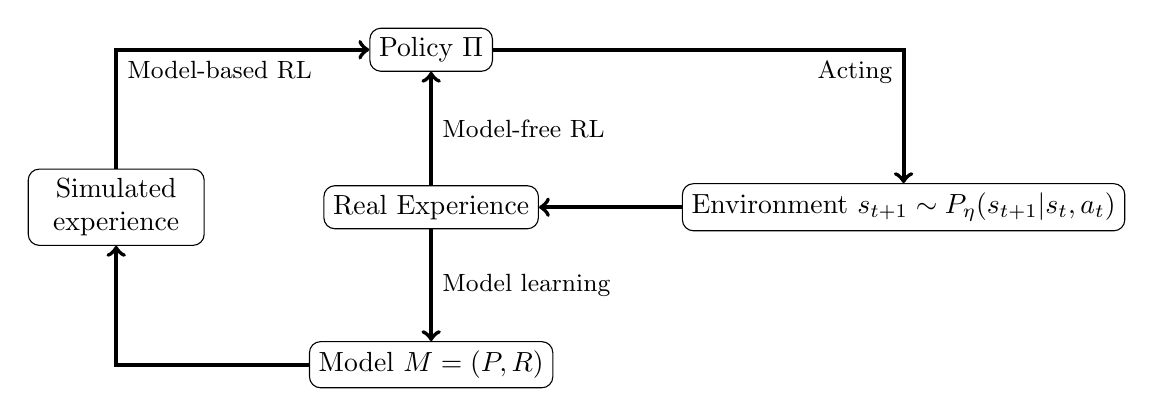
\begin{tikzpicture}[node distance=2cm]
        % Define nodes
        \node (policy) [rounded corners, draw] {Policy $\Pi$};
        \node (real_experience) [rounded corners, draw, below of=policy] {Real Experience};
        \node (environment) [rounded corners, draw, right of=real_experience, node distance=6cm] {Environment $s_{t+1}\sim P_\eta(s_{t+1}|s_t, a_t)$};
        \node (model) [rounded corners, draw, below of=real_experience] {Model $M = (P,R)$};
        \node (simulated_experience) [align=center, text width=2cm, rounded corners, draw, left of=real_experience, node distance=4cm] {Simulated experience};
        
        % Draw arrows
        \draw[->, line width=1.5pt] (policy) -| (environment) node[midway, below left, font=\small] {Acting};
        \draw[->, line width=1.5pt] (environment) -- (real_experience);
        \draw[->, line width=1.5pt] (real_experience) -- (model) node[midway, right, font=\small] {Model learning};
        \draw[->, line width=1.5pt] (model) -| (simulated_experience);
        \draw[->, line width=1.5pt] (real_experience) -- (policy) node[midway, right, font=\small] {Model-free RL};
        \draw[->, line width=1.5pt] (simulated_experience) |- (policy) node[font=\small, midway, below right] {Model-based RL};
    \end{tikzpicture}
    \caption{Model-free \ac{RL} vs. Model-based \ac{RL}}
    \label{fig:demo}
\end{figure}
% \tikzstyle{block} = [draw, fill=white, rectangle, 
%     minimum height=3em, minimum width=6em]
% \tikzstyle{sum} = [draw, fill=white, circle, node distance=1cm]
% \tikzstyle{input} = [coordinate]
% \tikzstyle{output} = [coordinate]
% \tikzstyle{pinstyle} = [pin edge={to-,thin,black}]

% \begin{tikzpicture}[auto, node distance=2cm,>=latex']

%     \node [input, name=input] {};
%     \node [sum, right of=input] (sum) {};
%     \node [block, right of=sum] (controller) {Controller};
%     \node [block, right of=controller, pin={[pinstyle]above:D},
%             node distance=3cm] (system) {System};

%     \draw [->] (controller) -- node[name=u] {$u$} (system);
%     \node [output, right of=system] (output) {};
%     \node [block, below of=u] (measurements) {Measurements};

%     \draw [draw,->] (input) -- node {$r$} (sum);
%     \draw [->] (sum) -- node {$e$} (controller);
%     \draw [->] (system) -- node [name=y] {$y$}(output);
%     \draw [->] (y) |- (measurements);
%     \draw [->] (measurements) -| node[pos=0.99] {$-$} 
%         node [near end] {$y_m$} (sum);
% \end{tikzpicture}

Typically, the model can be considered as a combination of state transition distribution $P_\eta$ and reward function $R_\eta$, $$M = (P,R) \textrm{ where } s_{t+1}\sim P_\eta(s_{t+1}|s_t, a_t) \textrm{ and } r_{t+1}\sim R_\eta(r_{t+1}|s_t, a_t)$$ $s_t$ is the state at time $t$, $r_t$ is the reward at time $t$ and $a_t$ is the action at time $t$. \ac{MBRL} learns an abstract model of the environment to plan the optimal policy. This model can be used to simulate the consequences of its actions, allowing it to make informed decisions, which makes it applicable to handle more complex environments, as it can make use of a model of the environment's dynamics. Therefore, model-based \ac{RL} requires a prior knowledge of the domainology\cite{tangModelbasedOnlineLearning2021}, as a model needs to be created and maintained. The domain of the model-based \ac{RL} refers to the context or environment in which the \ac{RL} agent is operating, which determines the available actions, observations, and rewards, and hence influences the behavior of the agent\cite{langExplorationRelationalDomains}. In model-based \ac{RL}, the agent needs to build a model of the dynamics of the system within the domain, and this model should accurately represent the true behavior of the system in order for the agent to learn effectively.

A data-driven approach for training the gait controller of a soft quadruped robot by \ac{MBRL} relies on the collection of empirical data to inform the control policy. However, this method presents various challenges, such as the need for specialized equipment and controlled experimental conditions, and may not be feasible in certain scenarios. Alternatively, a \ac{MBRL} approach employs a virtual model of the robot and its environment to generate training data in a rapid and cost-effective manner, thus enabling the exploration of diverse control policies and behaviors. This methodology offers advantages in terms of scalability and efficiency compared to a purely data-driven approach and is well-suited for training the gait controller of a soft quadruped robot. 

\subsection{Neural Network}

\section{Theory}
\ac{SAC} is a method
One approach to RL is model-based RL, where the agent learns a model of the environment dynamics and uses this model to plan its actions. Model-based RL has the potential to improve sample efficiency, which is crucial for robotics applications where data collection can be time-consuming and expensive. Model-based RL has been successfully applied to various robotics tasks, including manipulation and locomotion. However, the effectiveness of model-based RL depends on the accuracy of the learned model, which can be challenging to achieve in complex environments.

Several studies have investigated the use of model-based RL for quadruped robots. For example, Ha and Schmidhuber (2018) proposed an approach called world model-enhanced RL, where the agent learns a compact world model of the environment dynamics and uses it to plan its actions. They applied this approach to a simulated quadruped robot and achieved superior performance compared to other RL methods. Similarly, Chowdhary et al. (2020) proposed a model-based RL approach for quadruped robots that used a Gaussian process regression model to estimate the dynamics of the robot's locomotion. They demonstrated the effectiveness of their approach on a physical quadruped robot.

Soft robots have also been the subject of RL research. For example, Geijtenbeek et al. (2018) developed an RL-based controller for a soft robot arm that could grasp and manipulate objects. They used a model-free RL algorithm called deep deterministic policy gradient and demonstrated that the controller could adapt to different object shapes and sizes. Meanwhile, Yao et al. (2020) proposed a model-based RL approach for controlling a soft robotic arm with a cable-driven actuation system. They used a physics-based model of the arm and achieved superior performance compared to other RL methods.

Overall, the existing literature suggests that model-based RL has the potential to develop optimal policies for quadruped robots, including soft quadruped robots. However, the effectiveness of the approach depends on the accuracy of the learned model and the complexity of the environment. In addition, most existing studies have focused on simulated environments, and there is a need for further research on applying model-based RL to physical soft quadruped robots in real-world settings.
Each optimization algorithm supported by trainNetwork has its own advantages and disadvantages, and the choice depends on the specific problem and the network architecture. 

The process of modeling a robot is a fundamental step in developing an effective controller\cite{gromovModelingControlRobotic2019}. Modeling provides a means to understand the system's dynamics, which is crucial for designing controllers capable of precise control of the robot's locomotion. However, when it comes to soft legs with soft actuators, the modeling and control process becomes more challenging in comparison to rigid legs, which can be modeled using multi-body dynamics for their dynamic movements, This is due to the high non-linearity\cite{slotineAppliedNonlinearControl1991} and time variant properties\cite{wangControlStrategiesSoft2022} of soft materials, where the high non-linearity of soft materials makes them difficult to predict and control accurately, and the hysteresis and drift will introduce more unpredictable behaviors. Furthermore, the need to consider continuum mechanics, which deals with the behavior of continuously deformable materials with infinite \ac{DoF}\cite{polygerinosSoftRoboticsReview2017}, adds an extra level of complexity. Despite these challenges, some research groups from KTH Royal Institute of Technology\cite{jiSynthesizingOptimalGait2022,daneliaStructureGaitOptimizationof2021,thorapallimuralidharanContinuumActuatorBased2020,jiLearningbasedControl4D} have built a soft quadruped robot based on soft continuum actuators, which is capable of walking. Nonetheless, this robot does not move optimally, which highlights the need for further research and development in this area. This thesis work was based on the complete robot model developed by KTH Royal Institute of Technology.


\chapter{Methods and Methodologies}
\label{chap3}
% \thispagestyle{fancy}
\textit{This chapter motivates the methods and methodologies to answer the research questions.}
Describe the engineering-related contents (preferably with models) and the research methodology and methods that are used in the degree project. 

Most likely it generally describes the method used in each step to make sure that you can answer the research question.

\section{Methodologies}
Concerning \hyperref[rq1]{research question 1}, the state space restriction methods discussed should be confident to restrict the state space and increase the learning efficiency, since the algorithm is constructed directly from the state space, but the effectiveness of the surrogate model is undetermined. Therefore, an assessment of the effectiveness of the surrogate model is required, taking into account key metrics such as the Root Mean Squared Error (RMSE) of prediction on the gaits, Coefficient of determination ($R^2$) between simulations and predictions on the reference, and Normalized Root Mean Squared Error (NRMSE) of observations from the sensors on the robot. Then, the independent variables that will be used are settings of parameterization parameters, rotational angle $\alpha_r$, bending angle $\alpha_b$ and compressed length of the actuator $z_l$, which was determined by previous parameterization on the continuum actuators\cite{jiOmnidirectionalWalkingQuadruped2022}. Thus, dependent variables are simulation time, prediction accuracy and long-term prediction accuracy, where long-term prediction 
\begin{itemize}
    \item Independent variables: 
    \begin{itemize}
        \item Compressed length of the actuator limit($z_l$), Type: Continuous, Units: Millimeters
        \item Rotational angle ($\alpha_r$), Type: Continuous, Units: Radian
        \item Bending angle limit ($\alpha_b$), Type: Continuous, Units: Radian
    \end{itemize}
    \item Dependent variables:
    \begin{itemize}
        \item Model accuracy, Type: Continuous, Units: RMSE, $R^2$, RRMSE, Percentage
        \item Long-term prediction accuracy, Type: Continuous, Units: Percentage
        \item Simulation time, Type: Continuous, Units: Second
    \end{itemize}
\end{itemize}

After the data was collected, the data should be preprocess to conduct a correlation analysis to determine if there is a linear relationship between the independent variables and the dependent variable. To analyze the data, three multiple linear regressions will be conducted, with the three parameters as independent variables and each of performance metrics as the dependent variable. In addition, a best performane model should be determined from this test and proceed it to answer research question 2.
Regarding to \hyperref[rq2]{research question 2}, another ANOVA test could be conducted to evaluate the performance of model-based RL agent in comparison to model-free RL agent in terms of stability, walking speed and cost-of-transport. Firstly, the independent variables are defined as the desired walking speed and the type of RL method, with two levels: model-based RL and model-free RL. The dependent variables will be stability, walking speed, and cost of transport, measured as performance metrics during the gait. The stability of robot could be quantified by the zero-moment point (ZMP) method, while walking speed and cost-of-transport are direct performance metrics during gait. Data will be collected by simulating the gait controller using both RL methods, and measuring the three performance metrics for each simulation run, resulting in three data sets for each RL method. 
\begin{itemize}
    \item Independent variables: 
    \begin{itemize}
        \item Type of RL method, Type: Categorical, Units: Model-based, Model-free
    \end{itemize}
    \item Covariance:
    \begin{itemize}
        \item Desired walking speed ($v_x$), Type: Continuous, Units: Meter per second
    \end{itemize}
    \item Dependent variables:
    \begin{itemize}
        \item Stability, Type: Continuous, Units: Sum of moment, Newton*meter
        \item Resultant walking speed, Type: Continuous, Units: Meter per second
        \item Cost-of-transport, Type: Continuous, Units: Percentage
        \item Learning efficiency, Type: Continuous, Units: Number of iterations to converge
        \item Long-term planning , Type: Continuous, Units: Cumulative reward
    \end{itemize}
\end{itemize}
A one-way ANCOVA test will be conducted with RL method type as one factor, and the desired walking speed as a covariance. The null hypothesis is that there is significant difference in the means of the performance metrics between the two RL methods with different desired walking speed. If the null hypothesis is rejected, it indicates that there is a significant difference in at least one of the performance metrics between the two RL methods. The test bed is listed in Table \ref{tab:rq2test}. Furthermore, a Pareto analysis will be employed to evaluate the trade-off between multiple objectives, focusing on simulation benefits, where learning efficiency can be measured by the number of iterations or episodes required for the model-based RL algorithm to converge to a satisfactory policy, long-term planning effectiveness could be measured by evaluating cumulative reward obtained by the policy over a longer horizon. The Pareto front is then determined by identifying the set of solutions that cannot be improved in one objective without worsening at least one other objective. The Pareto set can be also computed, which is the set of algorithms that correspond to the Pareto front, and the Pareto optimal solutions will also be determined, which are the objective values associated with each point on the Pareto front. 
\begin{longtable}{|p{1cm}|cccccccc|}
\hline
    \multicolumn{1}{|c|}{\multirow{2}{*}{Method}} &
      \multicolumn{8}{c|}{\begin{tabular}[c]{@{}c@{}}Desired walking\\  speed $v_x$ (m/s)\end{tabular}} \\ \cline{2-9} 
    \multicolumn{1}{|c|}{} &
      \multicolumn{1}{c|}{0.01} &
      \multicolumn{1}{c|}{0.1} &
      \multicolumn{1}{c|}{0.3} &
      \multicolumn{1}{c|}{0.5} &
      \multicolumn{1}{c|}{0.75} &
      \multicolumn{1}{c|}{1} &
      \multicolumn{1}{c|}{1.5} &
      3 \\ \hline
    \endfirsthead
    %
    \endhead
    %
    Model-based RL &
      \multicolumn{1}{c|}{\begin{tabular}[c]{@{}c@{}}Test 1:\\ Test 2:\\ Test 3:\end{tabular}} &
      \multicolumn{1}{c|}{\begin{tabular}[c]{@{}c@{}}Test 1:\\ Test 2:\\ Test 3:\end{tabular}} &
      \multicolumn{1}{c|}{\begin{tabular}[c]{@{}c@{}}Test 1:\\ Test 2:\\ Test 3:\end{tabular}} &
      \multicolumn{1}{c|}{\begin{tabular}[c]{@{}c@{}}Test 1:\\ Test 2:\\ Test 3:\end{tabular}} &
      \multicolumn{1}{c|}{\begin{tabular}[c]{@{}c@{}}Test 1:\\ Test 2:\\ Test 3:\end{tabular}} &
      \multicolumn{1}{c|}{\begin{tabular}[c]{@{}c@{}}Test 1:\\ Test 2:\\ Test 3:\end{tabular}} &
      \multicolumn{1}{c|}{\begin{tabular}[c]{@{}c@{}}Test 1:\\ Test 2:\\ Test 3:\end{tabular}} &
      \begin{tabular}[c]{@{}c@{}}Test 1:\\ Test 2:\\ Test 3:\end{tabular} \\ \hline
    Model-free RL &
      \multicolumn{1}{c|}{\begin{tabular}[c]{@{}c@{}}Test 1:\\ Test 2:\\ Test 3:\end{tabular}} &
      \multicolumn{1}{c|}{\begin{tabular}[c]{@{}c@{}}Test 1:\\ Test 2:\\ Test 3:\end{tabular}} &
      \multicolumn{1}{c|}{\begin{tabular}[c]{@{}c@{}}Test 1:\\ Test 2:\\ Test 3:\end{tabular}} &
      \multicolumn{1}{c|}{\begin{tabular}[c]{@{}c@{}}Test 1:\\ Test 2:\\ Test 3:\end{tabular}} &
      \multicolumn{1}{c|}{\begin{tabular}[c]{@{}c@{}}Test 1:\\ Test 2:\\ Test 3:\end{tabular}} &
      \multicolumn{1}{c|}{\begin{tabular}[c]{@{}c@{}}Test 1:\\ Test 2:\\ Test 3:\end{tabular}} &
      \multicolumn{1}{c|}{\begin{tabular}[c]{@{}c@{}}Test 1:\\ Test 2:\\ Test 3:\end{tabular}} &
      \begin{tabular}[c]{@{}c@{}}Test 1:\\ Test 2:\\ Test 3:\end{tabular} \\ \hline
    
    
      \caption{ANCOVA tests examples for research question 2}
      \label{tab:rq2test}
\end{longtable}

Applying engineering related and scientific skills; modelling, analysing, developing, and evaluating engineering-related and scientific content; correct choice of methods based on problem formulation; consciousness of aspects relating to society and ethics (if applicable).

\section{Experiment Setup}


As mentioned earlier, give a theoretical description of methodologies and methods and how these are applied in the degree project.

\chapter{Model-based Reinforcement Learning}
\label{chap4}
\textit{This chapter reviews the details about the implementation of Model-based \ac{RL} for optimal gait control of soft quadruped robots by data-driven methods.}
\section{Neural Networks Design}
Describe the degree project. What did you actually do? This is the practical description of how the method was applied.

\section{Model-based RL Algorithm}

\section{Validation}
\chapter{Results}
\label{chap5}
\textit{This chapter presents the results of the experiments and evaluations conducted in this research. It provides a detailed analysis of the performance of MBRL algorithms with continuous training and provide insights into the research questions posed at the beginning of this study.}

\section{Surrogate Model Performance}
\subsection{Performance Evaluation}
To evaluate the surrogate model's performance, it is important to consider several critical metrics. These metrics serve as crucial indicators of how effectively the model approximates and forecasts the robot's behavior. Here, these metrics are elaborated without delving into details:
\begin{itemize}
    \item Average Steps before Failure: This metric assesses the model's capacity to predict the duration of a simulation run without encountering failure, serving as an indicator of sample efficiency.
    \item Validation RMSE and Validation Loss: This RMSE quantifies the disparity between the surrogate model's predictions and the actual values present in the validation dataset, as defined in Equation \ref{eq:RMSE}. Lower RMSE values are indicative of a higher degree of precision and accuracy in forecasting future states ($s_{t+1}$). Concurrently, the Validation Loss serves as an overarching measure of the model's performance on the validation dataset, underscoring the significance of minimizing this metric to enhance predictive capabilities, as defined in Equation \ref{eq:loss}.
    \item NRMSE: NRMSE provides a normalized measure of error, enabling comparisons of prediction accuracy across expert pattern datasets. It proves particularly valuable in evaluating the surrogate model's ability to predict sensor observations on the robot. The single step prediction NRMSE is calculated by Equation \ref{eq:NRMSE}, the long-term prediction NRMSE is calculated by Equation \ref{eq:NRMSET}.
    \item Correlation Coefficient ($R$): The $R$ quantifies the linear relationship between simulated and predicted values, as specified in Equation \ref{eq:R}. A higher $R$ signifies a more robust correlation, highlighting the model's proficiency in capturing underlying data trends and patterns.
\end{itemize}

\subsection{Control Variables Restriction}
The investigation commences with a focused exploration of state-space restriction within the surrogate model. The state-space, encompassing both observations and actions, is defined as $\mathbf{s}_t = [\pmb{\theta}(t), \mathbf{v}(t), \mathbf{f}n(t), \mathbf{a}_{t-1}]$ in Section \ref{sec:ss}. It is worth noting that the first three terms in this state-space originate from observations and are inherently challenging to restrict, but the action space can be subject to constraints.  It's crucial to acknowledge that the first three terms in this state-space comes from observations and present inherent challenges for restriction, but the action space can indeed be subjected to constraints. 

An important aspect to underscore is that the restriction of the robot's action space was achieved through the application of pattern-defined modeling techniques. Specifically, the robot's legs are interconnected in diagonal pairs, similar to a trotting pattern. This inherent structural arrangement significantly simplifies the action space compared to dealing with the complexity of controlling 12 individual motor actions\cite{jiSynthesizingOptimalGait2022}, effectively reducing it from $\mathbf{a}\in\mathbb{R}^{12}$ to $\mathbf{a}\in\mathbb{R}^4$. 

Furthermore, an alternate method of parameterization was applied, where the surrogate model's configuration incorporates specific control variables. Within this context, the actions are as defined in Section \ref{Sec:as}, taking the form of $\mathbf{a}_{t} = [\alpha_{b_1}, z_{l_1},\alpha_{b_2},z_{l_2}]$. These variables are subject to the bounds governed by the gains ($\alpha_{b_{gain}}\, , z_{l_{gain}}$). It's also crucial to emphasize that these gains associated with actions hold significance not only in the construction of the surrogate model but also play a vital role in shaping the behavior and adaptability of the SoftQ. Therefore, our focus centers on two key components within the action space: the gain of bending angle $\alpha_{b_{gain}}$ and the gain of compression length $z_{l_{gain}}$ for each of the diagonal leg pairs. To address this aspect, a series of simulations involving random actions within a bounded action space were carried out. These simulations aimed to gather the necessary data required for training the surrogate model. Subsequently, the performance of the trained model was evaluated. To effectively assess the trained neural networks performance, a color heat map can be employed to provide a visual representation of various performance metrics, as shown in Figure \ref{fig:NN_heat}. Each metric is associated with a specific color scale, allowing for a quick and intuitive evaluation.

\begin{figure}[htb]
    \centering
    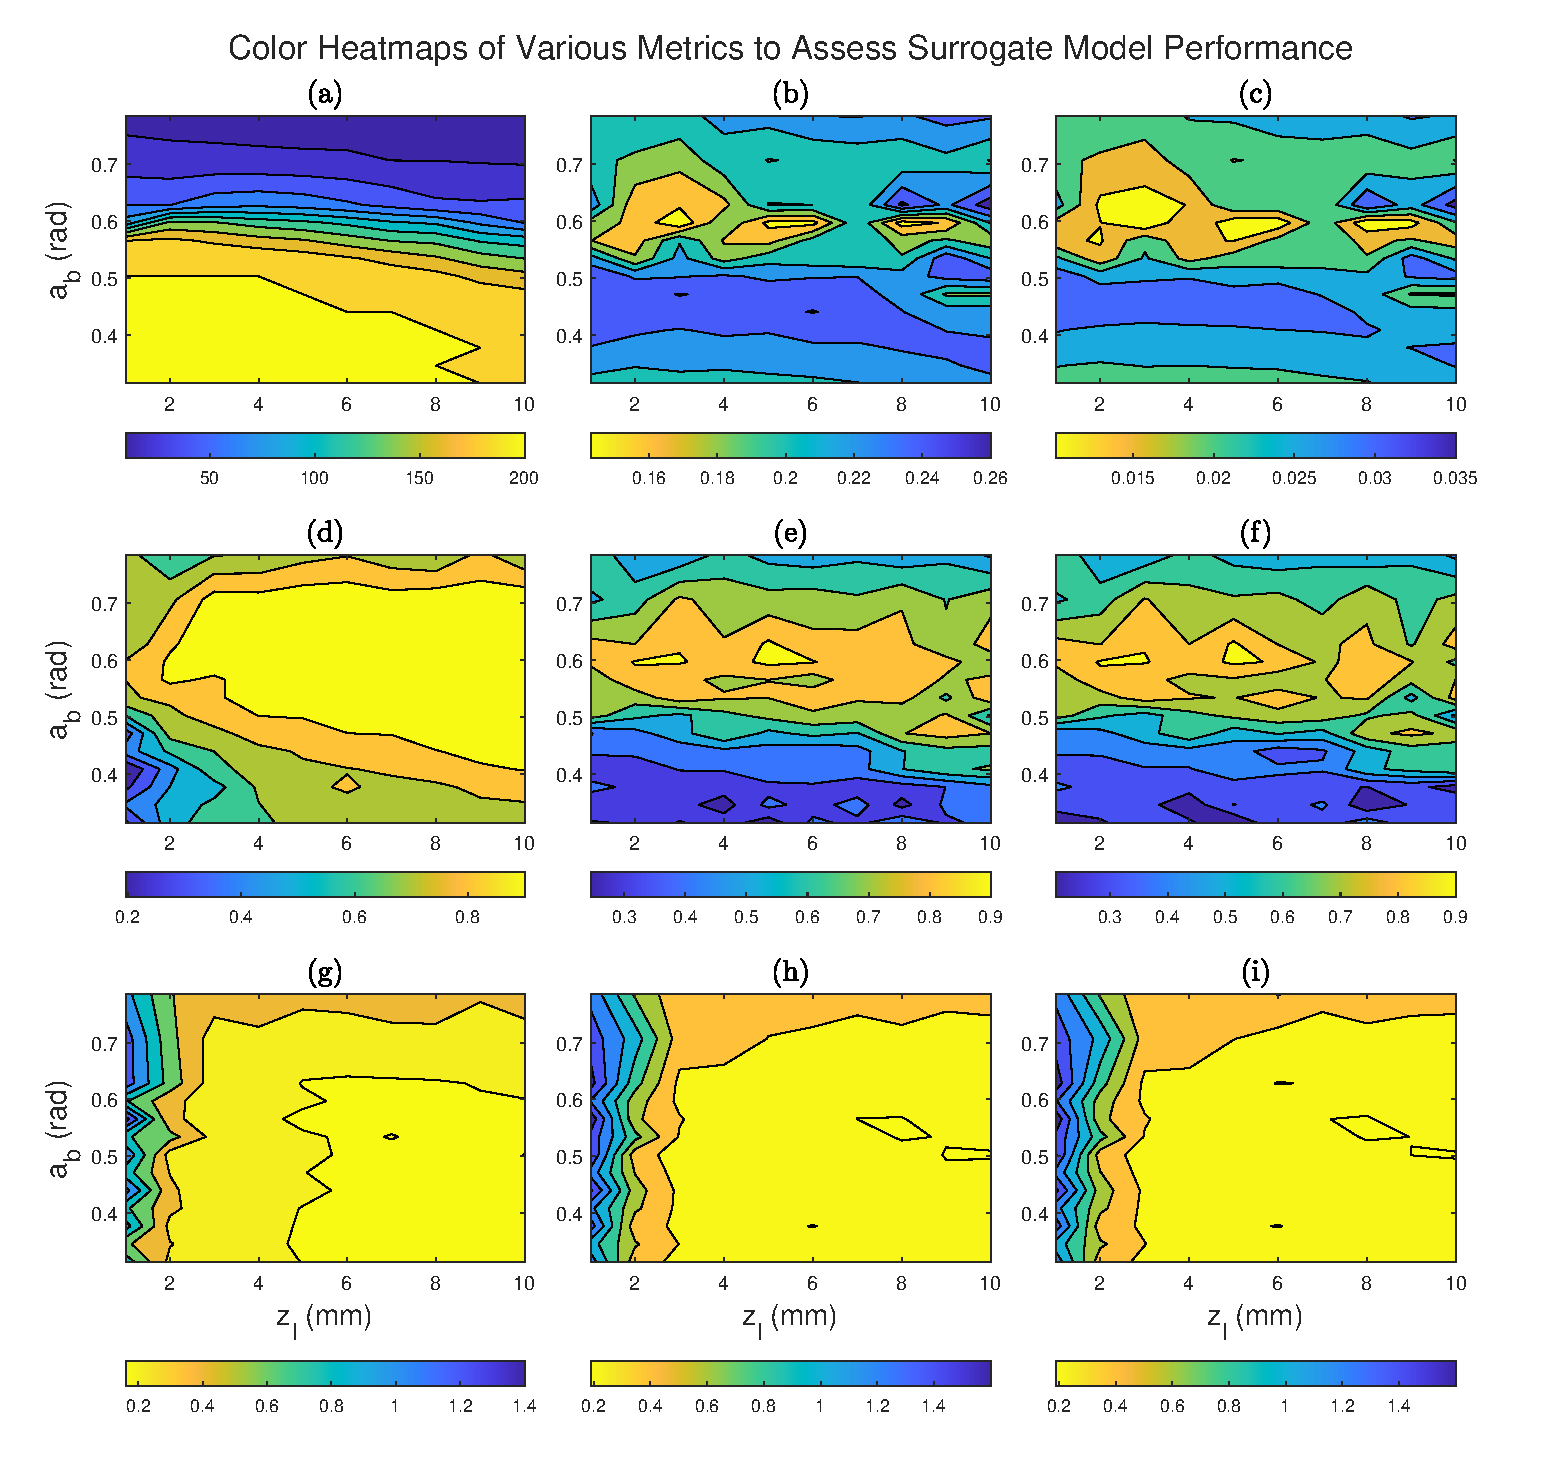
\includegraphics[width=\linewidth]{img/chap5/NN_heat.eps}
    \caption{Visualization of Performance Metrics Through Color Heat Map for Evaluating Trained Surrogate Models. The metrics include: (a) Average Steps before Failure; (b) \ac{RMSE} on the Validation Dataset; (c) Loss on the Validation Dataset; (d) Single Step Prediction Coefficient R; (e) Average Coefficient $R$ for Long-term Prediction; (f) Coefficient $R$ for Full Horizon Prediction; (g) NRMSE for Single Step Prediction; (h) Average NRMSE for Long-term Prediction; (i) NRMSE for Full Horizon Prediction.}
    \label{fig:NN_heat}
\end{figure}

In Figure \ref{fig:NN_heat}(a), it is evident that reducing the lower restrictions within the action space leads to an increase in the average number of steps the system can take before encountering failure, indicating improved data efficiency due to reduced locomotion risk with smaller actions. In Figure \ref{fig:NN_heat}(c), all neural networks converge with a loss below 0.037 in the validation dataset, with minimal differences between them. In Figure \ref{fig:NN_heat}(b), validated in the same dataset, RMSE converges to a minimum level. Notably, better validation RMSE is achieved when $\alpha_b$ ranges from 0.55 to 0.7 radians and $z_l$ ranges from 3 to 9 millimeters, suggesting optimal model performance within these parameter ranges.

In assessing single-step predictions using various expert gait pattern datasets, the correlation coefficient ($R$) between predictions and ground truth was calculated, as depicted in Figure \ref{fig:NN_heat}(d). The results show consistently high accuracy when either the compression length ($z_l$) or the bending angle ($\alpha_b$) is high, or when both are elevated. This observation aligns with the expectation that for the robot to achieve higher speeds, it should exhibit more pronounced behaviors, which are characterized by larger values of these parameters. Consequently, the expert gait dataset used in this context emphasizes high values of $\alpha_b$ and $z_l$, resulting in smaller differences between predictions and ground truth, and consequently, lower values of R. A similar trend is observed when considering single-step predictions. Smaller NRMSE values are associated with high values of $z_l$ and $\alpha_b$, but interestingly, low $\alpha_b$ values also yield small NRMSE values. This implys that bending angle ($\alpha_b$) exerts a more significant influence on robot locomotion. These results are visually represented in Figure \ref{fig:NN_heat}(g). However, it is important to note that neither the NRMSE nor $R$ reach their lowest points in the highest $\alpha_b$ region, suggesting poorer predictions when too small steps are taken before simulation failure, resulting in an insufficient amount of useful data.

For multi-step predictions on the same expert gait pattern datasets, the effects of $\alpha_b$ and $z_l$ are similar in single step prediction, but the models with low $\alpha_b$ values perform less effectively in predicting over longer time horizons, suggesting a lack of robust generality in these models. However, as shown in Figure \ref{fig:NN_heat}(e), the average correlation coefficient ($R$) for long-term predictions reveals that models with relatively high values of both $\alpha_b$ and $z_l$ struggle to predict states over extended horizons. This challenge could be attributed to the larger action space, which introduces more unpredictability and subsequently leads to reduced performance compared to models with lower $z_l$ values when trained on the same dataset size. This trend is also evident in the full horizon prediction R, as depicted in Figure \ref{fig:NN_heat}(f), where predictions at relatively high values of both $\alpha_b$ and $z_l$ deteriorate. In addition, the average NRMSE of long-term predictions exhibits a similar performance to what was observed in single-step predictions, which shows different patterns compared to $R$ results, because the NMRMSE is normalised and large values like contact forces may have more effects on the metrics. Lower errors are associated with larger values of $\alpha_b$ and $z_l$, but NRMSE also decreases when $\alpha_b$ reaches its highest values. These results are presented in Figure \ref{fig:NN_heat}(h). Interestingly, performance remains consistent when $\alpha_b$ is smaller than 0.72 radians and $z_l$ is larger than 3 millimeters. Likewise, in the case of NRMSE for full horizon prediction, there is no significant change in performance, as indicated in Figure \ref{fig:NN_heat}(i).

Hence, the optimal action state restrictions can be identified as approximately $\alpha_b$ around 0.6 rad and $z_l$ around 7 mm. However, it's important to consider that these restrictions also impact MBRL training, as they limit the range of exploration within the robot's action space. Therefore, it's preferable to keep the action space as broad as possible. Another viable set of restrictions to consider is $\alpha_b$ around 0.63 rad and $z_l$ around 8 mm for the state space during surrogate model training and MBRL training. This broader range allows for more exploration and potentially better overall performance in subsequent MBRL learning.

\section{Model-based RL Training}
After the surrogate model determined in Section \ref{sec:NN_design}, we can continue to training of MBRL for optimal gait controls, which will be used as a gait controller in robot to navigate with learned optimal gait. It's important to note that the training settings remained consistent across all experiments. The code snippet for training details can be found in Section \ref{code:mbrl}. To account for potential variations due to randomness, the training process was initiated with various random seeds. It was observed that training had a higher failure rate when the agent became trapped in local minima. Consequently, it can be intuitively inferred that mastering the policy for low-speed locomotion posed a more challenging task for the agent. Notably, in the experiments, $v_{ref}$ was maintained at no smaller than 0.1 m/s to ensure meaningful training outcomes and the final time of the training in one episode $T_f$ is 10 seconds.
\begin{figure}[htb]
    \centering
    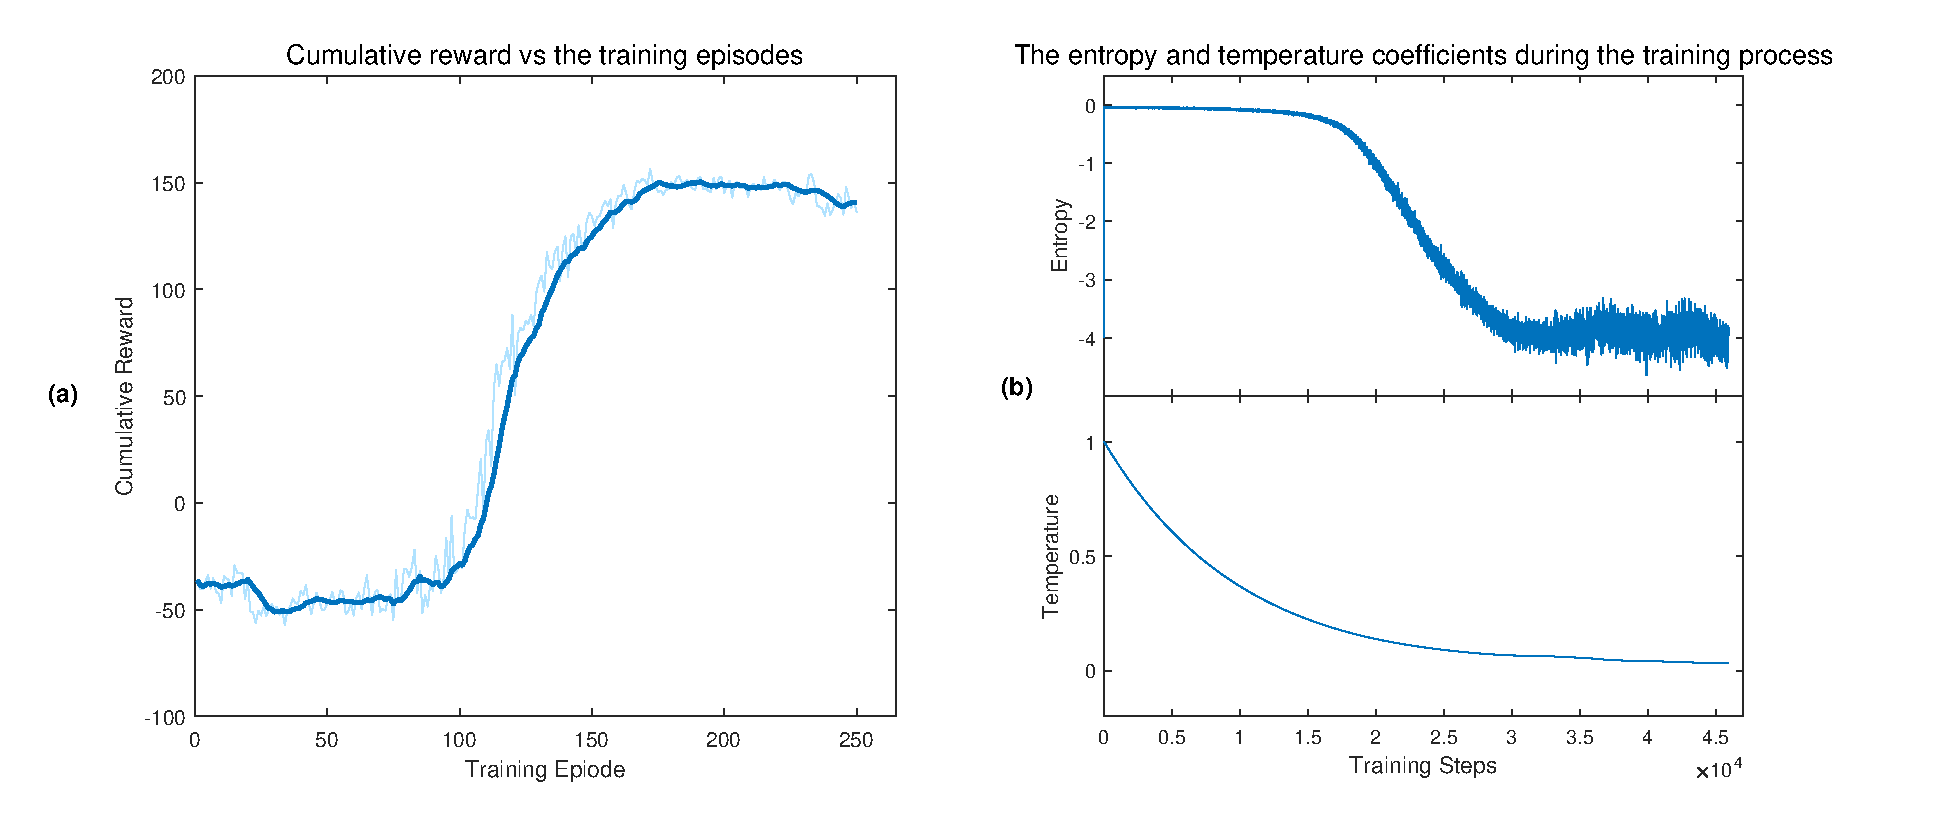
\includegraphics[width=\linewidth]{img/chap5/MBRL_tr.eps}
    \caption{The Training Results of MBRL. (a) Cumulative reward in MBRL vs the training episodes; (b) The variation of entropy and temperature parameters during the training process.}
    \label{fig:MBRL_tr}
\end{figure}

The training progress, along with the entropy and temperature parameters, is visually represented in Figure \ref{fig:MBRL_tr}. The plot illustrates the successful training of the agent using the SAC algorithm. The cumulative reward steadily increased from approximately -45 to 150, indicating the acquisition of the desired behavior by the agent. Additionally, the entropy decreased to around -4 (with the goal being the negative of the number of actions), and the temperature parameter also exhibited a decline from 1 to 0.05. These trends signify that the agent effectively learned the desired behavior during the training phase. Subsequent to the training process, the trained agent was implemented in simulation to evaluate its performance. The results of this implementation are elucidated in Figure \ref{fig:MBRL_val}, providing valuable insights into how well the trained MBRL model performs in executing optimal gaits for the SoftQ. 

Post-training validation in the simulation environment, conducted for a duration of 5 seconds, yielded noteworthy observations. As depicted in the figure, the robot exhibited some velocity along the x-axis. However, it remained virtually stationary at its initial position, effectively patrolling within a confined area. Despite generating speed, the robot failed to manifest any significant forward displacement. This phenomenon is notably characterized by a marked increase in the \ac{COT} during the initial phases of robot motion. This surge in \ac{COT} can be attributed to the imperative need for the robot to surmount inertia and initiate acceleration as it commences motion. Consequently, a substantial input of energy is necessitated. Additionally, heightened frictional forces encountered by mechanical components, such as wheels and joints, during the initial moments of motion contribute to this increased energy expenditure.

\begin{figure}[htb]
    \centering
    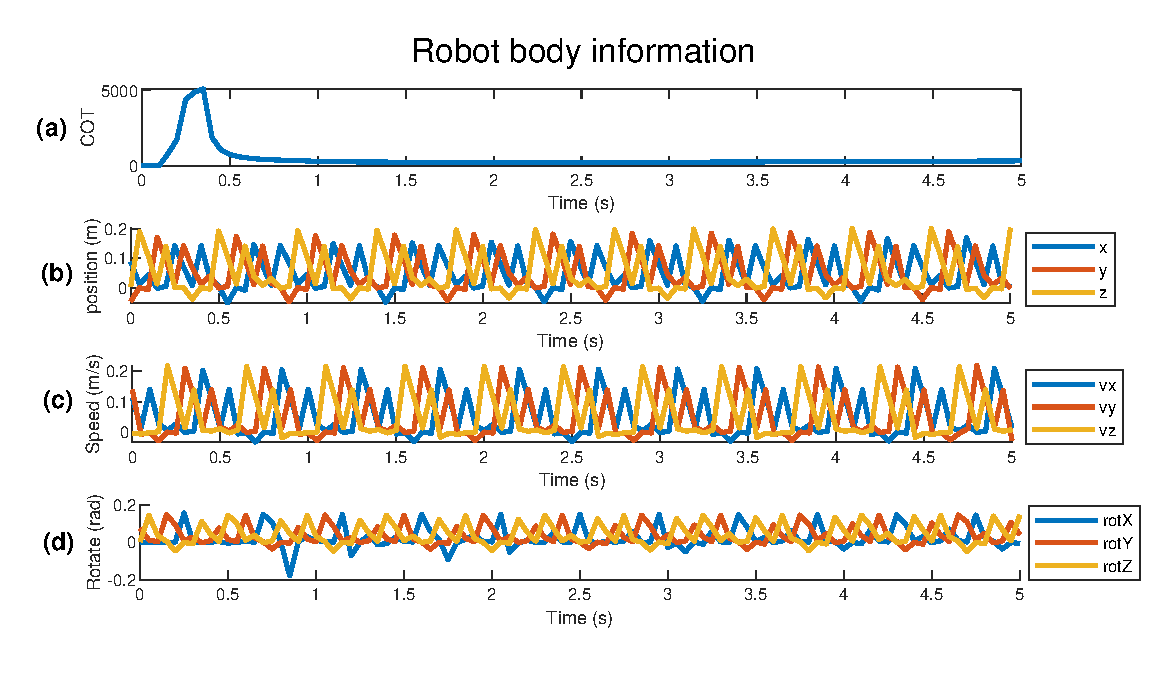
\includegraphics[width=\linewidth]{img/chap5/MBRL_val.eps}
    \caption{The Validation Results of MBRL. (a) COT of the robot while walking; (b) Distance traveled along the $x$, $y$, and $z$ axis; (c) Speed of the robot along the $x$, $y$, and $z$ axis; (d) Orientation of the robot along the $x$, $y$, and $z$ axis.}
    \label{fig:MBRL_val}
\end{figure}

To assess the operational capacity and explore the gait patterns of the soft robot, the same RL configurations were applied to learn optimal gaits under different reference speeds denoted as $v_{ref}$. Throughout the training experiments, an interesting observation emerged: the training performance of the simulated robot was notably influenced by the reference speed $v_{ref}$. When the target velocity was set higher, the learning agent was able to achieve forward motion in fewer training episodes, ultimately converging to an effective policy. Conversely, when $v_{ref}$ was set to a lower value, the agent exhibited a tendency to pitch forward, resulting in episode termination. The training process was initiated with various random seeds, and it was observed that training had a higher failure rate when the agent became trapped in local minima. Consequently, it can be intuitively inferred that mastering the policy for low-speed locomotion posed a more challenging task for the agent.

Given the limitations observed in the direct application of the agent trained through MBRL, a decision was made to further train this agent in a model-free environment to bridge the reality gap effectively. It is noteworthy that adjustments were made to the reward structure, particularly in penalizing instances where all four legs bent in the same direction with a significant angle. The coefficient $\epsilon_4$ governing this penalty was increased from 10 to 100. This modification was introduced due to the possibility that the model-based training might generate actions that are fatal in simulation but less perilous in the real-world scenario.

\subsection{Continue Learning}
To accelerate the training process, a predefined expert behavior, denoted as $A^e = [\textbf{a}_{T_0}^e, ..., \textbf{a}_T^e]$, is established\cite{jiSynthesizingOptimalGait2022}. This predefined behavior offers the robot an initial stable gait. Specifically, during the initial second of each training episode, the RL agent emulates human knowledge by executing the predefined behavior $A^e$. By this means, we resort to the framework of \textit{imitate learning}\cite{koberImitationReinforcementLearning2010}. Data generated from this process is collected and stored in a replay buffer for subsequent learning phases. This approach aligns with the principles of imitation learning, where the RL agent imitates pre-established behaviors as a form of guidance. While it is important to note that this predefined state-action trajectory does not guarantee the optimality, it serves as a valuable reference for the agent. Emulating these guided elementary movements enables the agent to swiftly implement and adapt its behavior in real-time scenarios, contributing to efficient online implementation. 

To continue training the agent from MBRL, the same RL configurations were applied, with the exception of the penalty adjustment for the four legs bending. The goal for the robot was to learn an optimal gait for higher speed, with $v_{ref}$ set at 0.3 m/s. The reward functions remained the same as defined in Equation \ref{eq:reward}, but the coefficients were adjusted to $[\epsilon_1, \epsilon_2, \epsilon_3, \epsilon_4, \epsilon_5] = [5, −1/v_{ref}, 0.25, 100, 3]$. 

The results of continuous training are visualized in Figure \ref{fig:MFRLvsCT} for comparison with Model-Free Reinforcement Learning (MFRL). Notably, it is observed that the continuous training policy exhibited rapid improvement, reaching convergence at around 200 episodes. However, it's important to note that this policy incurs higher penalties, aligning with the assumption that the MBRL policy may generate riskier actions. Additionally, the MFRL policy converges at approximately 120 episodes, which is slower than the continuous training agent. However, the reward at the beginning of training is higher for MFRL, indicating that the agent in early training may not actively promote forward motion but is associated with fewer high-risk actions. Furthermore, the MFRL approach failed to converge to a walking gait even after 350 episodes, and the MFRL agent did not learn to travel a significant distance. Notably, the MFRL method required about 24 hours of training, while MBRL and continuous training together took approximately 10.5 hours. This substantial reduction in training time, coupled with the ability to achieve effective learning and improved gait control, underscores the efficiency and effectiveness of the continuous training approach compared to the benchmark MFRL method.
\begin{figure}[htb]
    \centering
    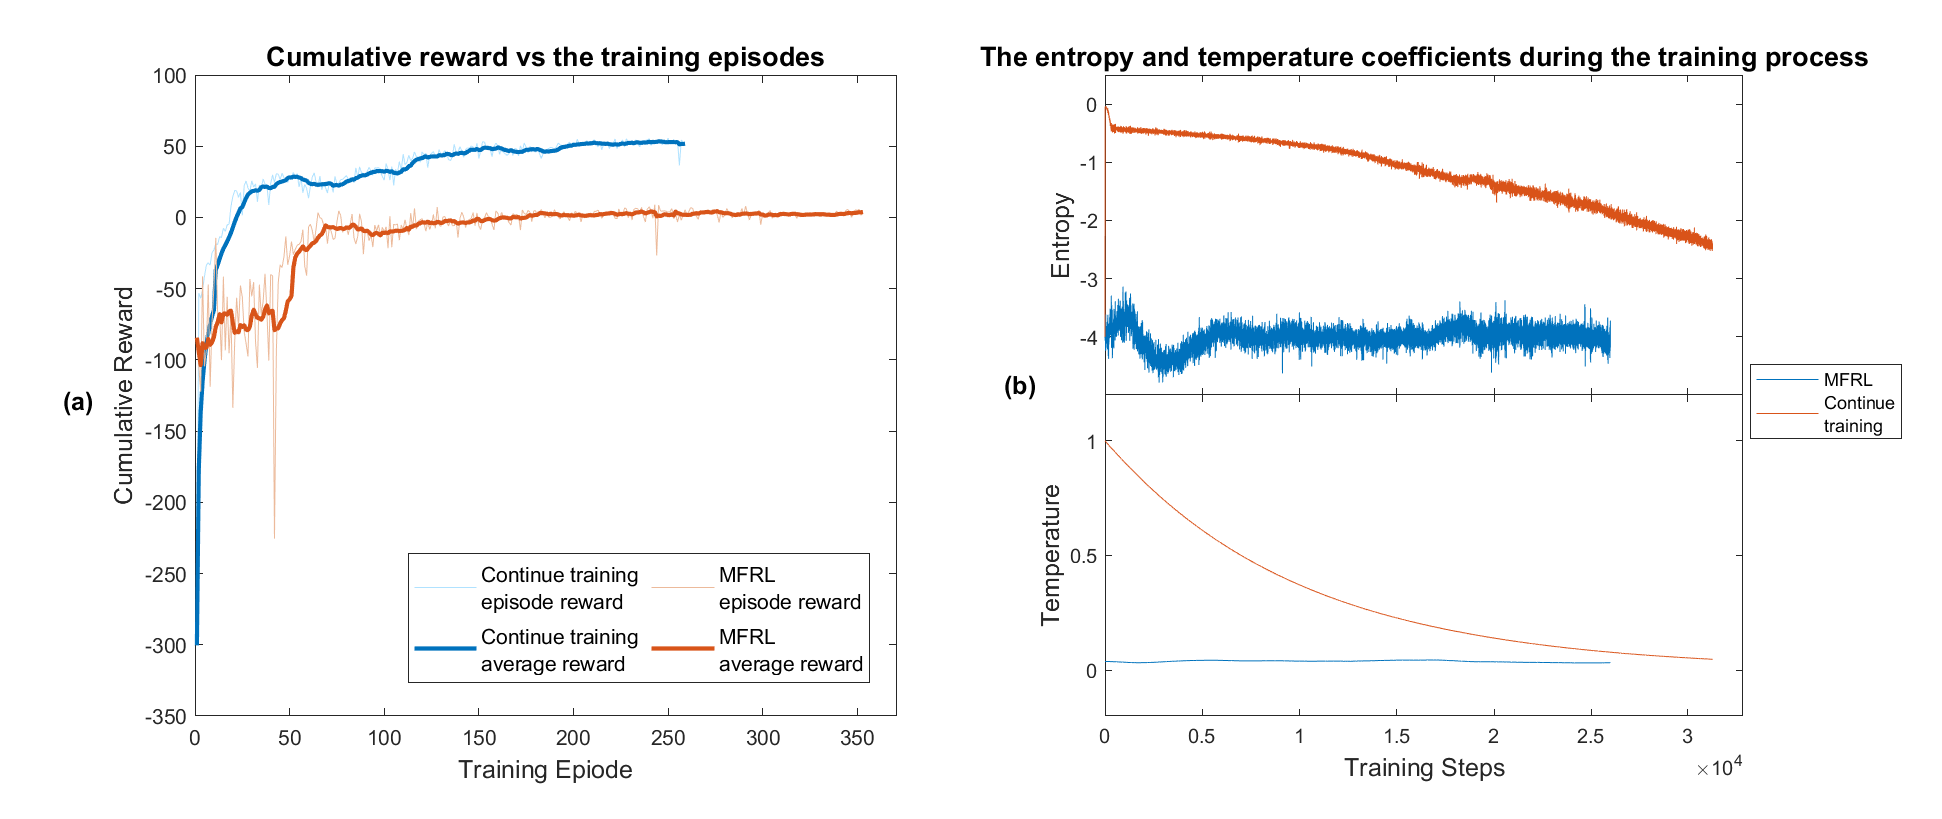
\includegraphics[width=\linewidth]{img/chap5/MFRLvsCT.eps}
    \caption{The Training Results of Continuous Training Compared to MFRL. (a) Cumulative reward in MFRL and continuous training vs the training episodes; (b) The variation of entropy and temperature coefficients during the training process of both MFRL and continuous training.}
    \label{fig:MFRLvsCT}
\end{figure}

The outcomes of validations for continuous training are graphically presented in Figure \ref{fig:CT}, which serves as a overview of continuous training performance. The COT achieved a remarkable low value of approximately 73 J/kg/m, signifying the robot's ability to traverse a certain distance with efficient energy consumption. However, it's worth noting that at the beginning of movement, the COT exhibited a notable increase, reaching approximately 200 J/kg/m. This initial rise in COT can be attributed to several factors, such as static friction, initiate acceleration, and control and actuator-related challenges during the transition from rest to motion. Despite this initial increase in COT, the robot demonstrated its capability to efficiently attain and sustain a speed higher than the predefined benchmark $v_{x_{avg}}$ = 0.2 m/s, as attached in Appendix Figure \ref{fig:expert_val}. Over a 5-second validation period, the robot covered a distance of 1.8 meters, achieving an average speed of 0.36 m/s, surpassing the reference speed $v_{ref}$ of 0.3 m/s. These findings highlight the agent's capability to attain and sustain a speed higher than the predefined benchmark. Moreover, the robot demonstrated stability during locomotion, as indicated by the minor fluctuations in velocity along the $x$-axis and minimal deviations in the $y$ and $z$ axes. The orientation plots revealed controlled movement, with the largest rotation measuring approximately 0.055 radians in the initial stages, confirming a stable and well-maintained gait. Collectively, these validation results underscore the practical viability of the continuous training technique in enhancing the robot's performance in real-world scenarios.

\begin{figure}[htb]
    \centering
    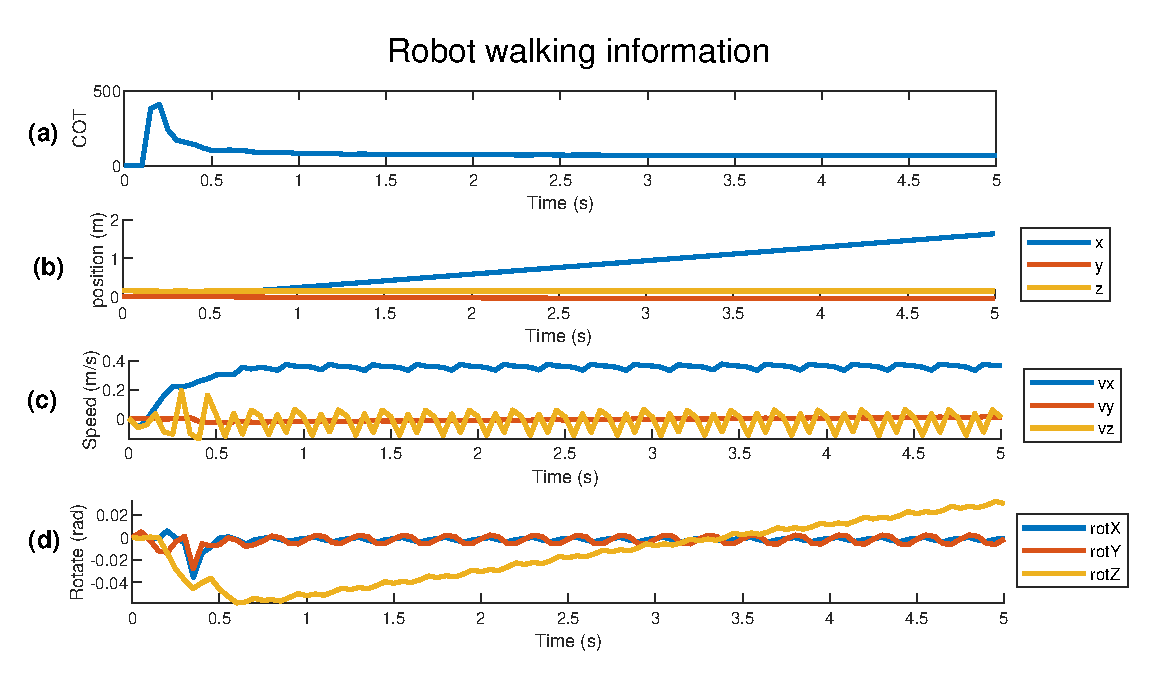
\includegraphics[width=0.9\linewidth]{img/chap5/best_CL.eps}
    \caption{The Validation Results of Continuous Training. (a) COT of the robot while walking; (b) Distance traveled along the $x$, $y$, and $z$ axis; (c) Speed of the robot along the $x$, $y$, and $z$ axis; (d) Orientation of the robot along the $x$, $y$, and $z$ axis.}
    \label{fig:CT}
\end{figure}

Figure \ref{fig:CT_gait} (a) shows the examples of the four foot trajectories, and Figure \ref{fig:CT_gait} (b) with colored areas representing the contact regions demonstrates a typical gait patterns captured from the validation simulation. Synchronized motions were observed between the FR and RL legs, as well as the FL with RR legs, as they are linked as pairs. Notably, the FL and RR leg pairs exhibit a smaller swing area compared to the FR and RL pairs. This difference in swing area may be attributed to corrective actions addressing yaw rotation errors. These yaw rotation errors could potentially be caused by slight uneven mass distribution on the robot, favoring the right side, as indicated by the orientation in the $z$ axis shown in Figure \ref{fig:CT} (d). Additionally, a delay of approximately 0.1 seconds is observed between each diagonal leg pair. The contact time for each leg is around 0.15 seconds, resulting in the formation of a periodic gait pattern. This pattern indicates that the robot successfully learned to coordinate its movements in a rhythmic manner, which is essential for stable and sustained locomotion.

\begin{figure}[htb]
    \centering
    \begin{subfigure}[b]{0.45\textwidth}
    \centering
    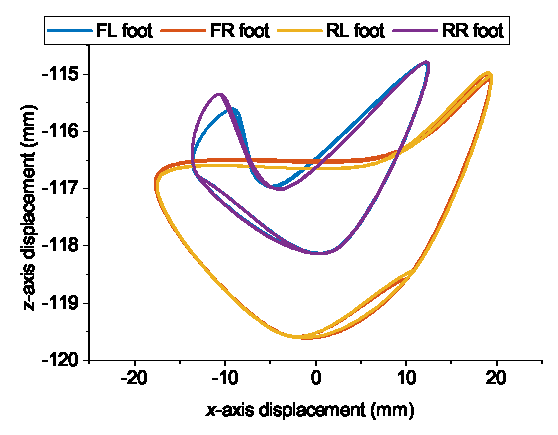
\includegraphics[width=\linewidth]{img/chap5/foot_trace.eps}
    \caption{}
    \end{subfigure}
    \begin{subfigure}[b]{0.45\textwidth}
    \centering
    \includegraphics[width=\linewidth]{img/chap5/pattern.pdf}
    \caption{}
    \end{subfigure}
    \caption{The Learned gait patterns. (a) Four foot moving trajectories. (b) Footfall patterns}
    \label{fig:CT_gait}
\end{figure}

Moreover, it's essential to highlight that the observed results go beyond demonstrating successful gait patterns and stability. They also reveal the practical significance of this achievement in terms of direction control within velocity control. As shown in Figure \ref{fig:CT} (d), in the beginning of walking, the robot initially turns to the right but subsequently corrects itself, adjusting its orientation slightly to the left by the end of the gait cycle. This phenomenon was also observed in field tests, as presented in Section \ref{video}. This capability for self-correction and precise direction control enhances the robot's suitability for applications that require controlled and accurate movement, further expanding its utility in real-world scenarios. 

\section{Model-based RL Comparison}
\label{Sec:MBRL}
Given that the MBRL with continuous learning reached a superior performance than MFRL in the same experimental setting; however, it is still required more examinations to statistically prove that MBRL with continuous learning suppress MFRL. Therefore, to establish the statistical significance of this observation and confirm that MBRL with continuous learning outperforms MFRL consistently, further comprehensive examinations are required. This section aims to systematically and statistically determine which RL method is more effective for optimally controlling the gait of a soft quadruped robot. 

\subsection{Performance Evaluation}
In the performance evaluation of the trained agent, it is important to consider several critical metrics, which have been discussed in Section \ref{Sec:test_def}. These metrics serve as crucial indicators of proficiency of the agent, referred to as the controller. Here, these metrics are expounded again avoiding excessive details:
\begin{itemize}
    \item Stability: This metric combines information about the time duration of the gait, rotational motion, and vertical displacement to assess the stability of the gait. It is calculated using Equation \ref{eq:stability} and provides valuable insights into the agent's ability to maintain stability during operation. 
    \item Resultant walking speed (m/s): This metric involves assessing the agent's walking speed, particularly by calculating the average speed achieved during validation. It offers a straightforward measure of the agent's mobility and effectiveness in movement.
    \item Cost-of-Transport (J/kg/m): The COT metric evaluates the energy efficiency of the agent. It is defined in Equation \ref{eq:COT} and quantifies quantifies the amount of energy expended by the agent, normalized by its weight and the distance traveled. This metric is crucial for understanding the agent's energy consumption patterns.
    \item Learning efficiency: Learning efficiency gauges how quickly the agent converges to an optimal or satisfactory performance level. It is quantified by measuring the training time required for the agent to reach convergence and the reward reach a significant level. This metric provides insights into the agent's adaptability and learning capabilities.
\end{itemize}

\subsection{Compare with MFRL}
This section will delve into the performance comparison between the MBRL with continuous training and MFRL based metrics outlined earlier. To ensure a robust evaluation, three identical training sessions were conducted for each reference velocity $v_{ref}$, which took values of 0.2 m/s, 0.3 m/s, and 0.5 m/s. Training was stopped upon the convergence of each policy to a significant reward level. Following the training phase, each trained agent was implemented and evaluated through simulation of 5s. The results of these evaluations are visually represented in Figure \ref{fig:box}. It is evident from the figure that MBRL with continuous training consistently outperforms MFRL. This conclusion is drawn based on the observation that the mean values of key performance metrics, including stability, resultant walking speed, COT, and training time, are consistently higher for MBRL with continuous training compared to MFRL. 

Specifically, in terms of stability, MBRL with continuous training achieved a mean stability level of approximately 0.62, significantly surpassing MFRL, which achieved a mean stability of approximately 0.05. Notably, the level of stability achieved by MBRL with continuous training closely approximated that of the predefined expert gait, indicating its capability to generate highly stable locomotion. 
\begin{figure}[htb]
    \centering
    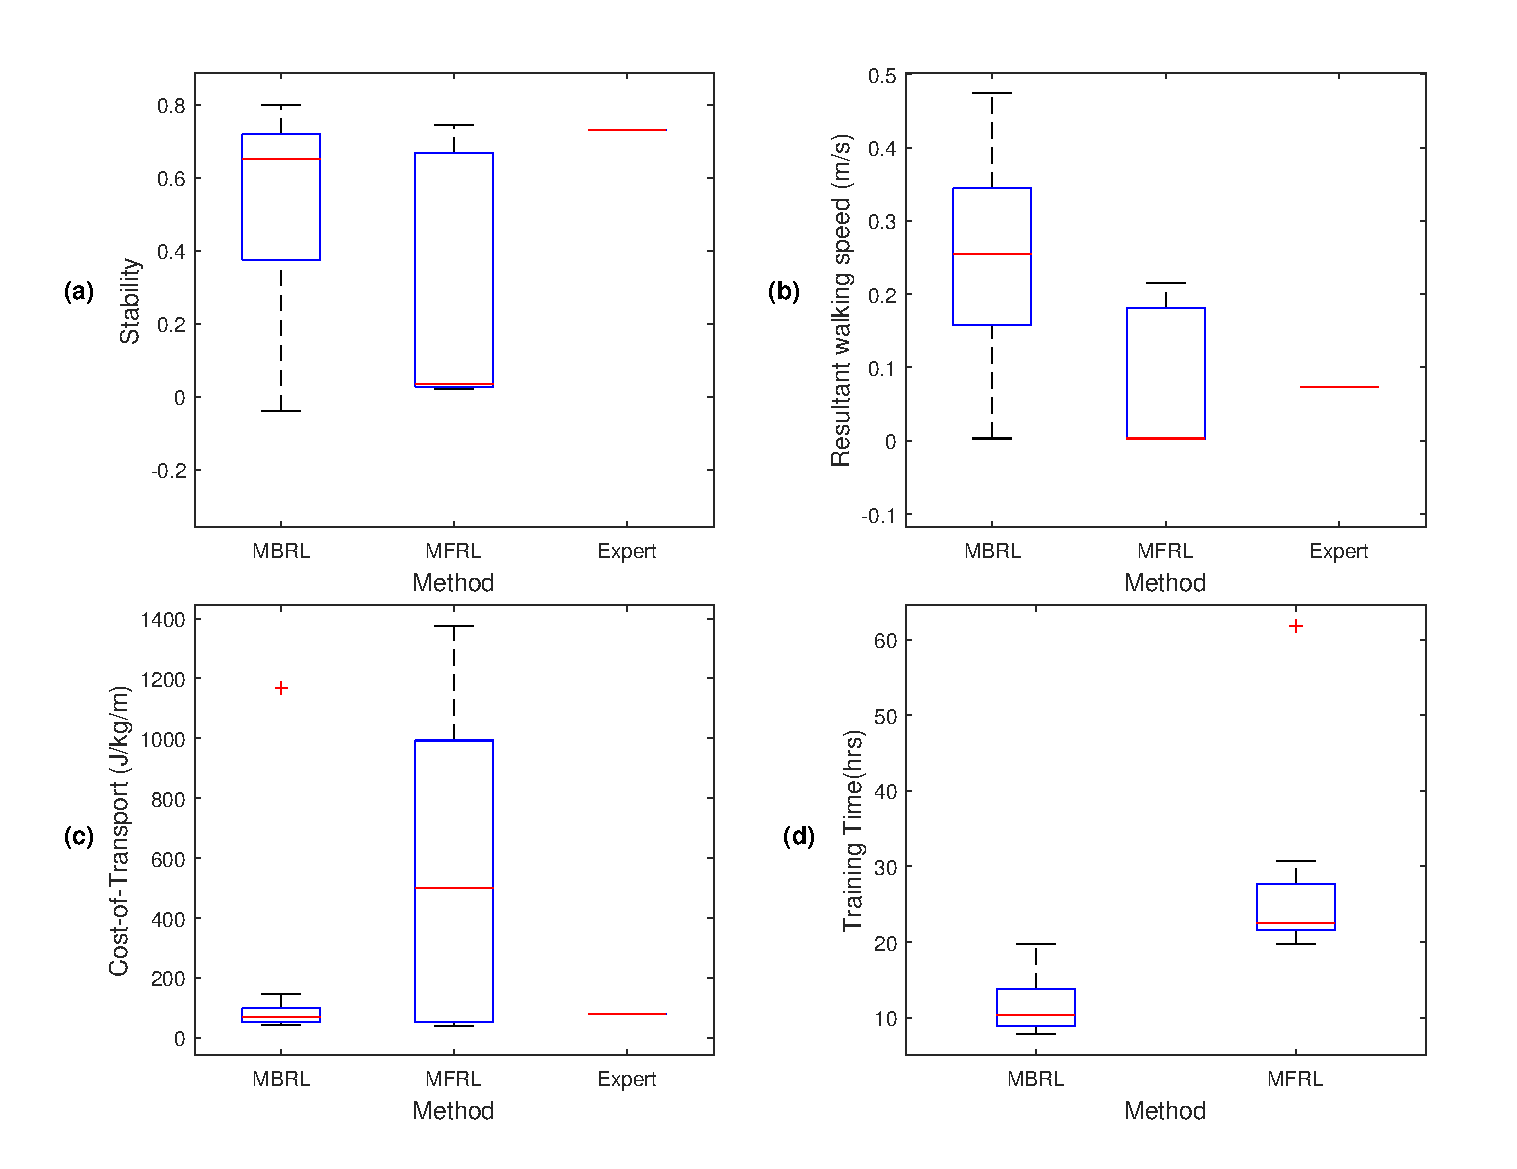
\includegraphics[width=\linewidth]{img/chap5/box_results.eps}
    \caption{The Box Plot of MBRL with Continuous Training compared to MFRL. (a) Box plot of stability by method; (b) Box plot of resultant walking speed by method ; (c) Box plot of COT by method; (d) Box plot of simulation time by method.}
    \label{fig:box}
\end{figure}

Regarding resultant walking speed, it was noted that MBRL with continuous training exhibited a higher mean walking speed. However, it also displayed a larger variance, partly due to variations in reference walking speeds ($v_{ref}$).Despite the variance, the mean walking speed achieved by MBRL with continuous training was significantly greater than that of MFRL. It's worth noting that MBRL, in its pursuit of efficient locomotion, tended to focus on walking further, resulting in a mean speed that was significantly higher than the expert gait's speed, even though it initially learned from the expert gait. In contrast, MFRL faced challenges in learning extended walking within 350 training episodes, which is reflected in the mean speed approaching zero. It primarily struggled to adapt and achieve higher speeds or longer distances. This disparity in performance between MBRL with continuous training and MFRL underscores the advantages of the former approach in facilitating both stable and efficient locomotion, even surpassing the performance of the expert gait. 

Furthermore, the analysis revealed that MBRL with continuous training achieved an efficient COT level, similar to that of the predefined expert gait, indicating economical energy consumption during locomotion. In contrast, MFRL agents exhibited significantly higher COT values. This difference primarily stemmed from the fact that only a limited number of MFRL agents succeeded in overcoming the initial resistance associated with initiating longer-distance walking. 

Lastly, it was observed that MBRL with continuous training demonstrated superior training efficiency, aligning with the primary objective of this thesis. It exhibited a greater capacity to learn efficient locomotion, particularly for longer distances. Additionally, considering that a smaller fraction of MFRL agents achieved extended walking within 400 episodes, the actual simulation time required for MFRL to achieve comparable results would likely exceed what is presented in Figure \ref{fig:box}(d).

In summary, the findings emphasized the consistent advantages of employing MBRL with continuous training over MFRL in terms of stability, walking speed, energy efficiency, and training effectiveness. Furthermore, MBRL with continuous training not only outperforms MFRL but also attains performance levels similar to those of the predefined expert gait, showcasing its potential for real-world applications where stable and efficient locomotion is of paramount importance.

\subsection{ANCOVA Tests}
However, it is essential to acknowledge that reference walking speed ($v_{ref}$) represents a covariate in this comparative analysis. To ensure a rigorous assessment that accounts for the potential influence of this covariate, an \ac{ANCOVA} was conducted to compare MBRL with continue learning and MFRL. This statistical analysis enabled us to compare these two RL approaches while effectively controlling for the covariate $v_{ref}$. This analysis primarily focused on the following dependent variables, as previously defined in Section \ref{Sec:test_def}: stability, resultant walking speed, COT and learning efficiency. This ANCOVA analysis provides a robust framework for evaluating the relative performance of the two RL approaches, while considering the potential impact of reference walking speed ($v_{ref}$). The results of this analysis offer deeper insights into the effectiveness of each method in achieving stable and efficient gait control for our soft robot. The details of ANCOVA is discussed in \ref{Sec:ANCOVA}.

The hypothesis holds that MBRL with continuous training is significantly more effective and efficient in achieving stable and efficient gait control for our soft robot SoftQ compared to MFRL, across various reference velocities ($v_{ref}$).

\subsubsection*{Stability}
The ANCOVA analysis revealed both the method of RL (MBRL or MFRL) and the covariate $v_{ref}$ have a statistically significant effect on walking stability. The F-value of 5.9902 and the p-value of 0.0307 in the effect of method indicate that the method of RL significantly influences walking stability. Given that the p-value is less than 0.05, this effect is statistically significant, suggesting that one of these methods is likely better than the other in terms of enhancing walking stability. $v_{ref}$ serves as a covariate in this study, and it too shows a statistically significant F-value of 4.3583 and a p-value of 0.0378. This implies that $v_{ref}$ independently impacts walking stability, and its effect is statistically significant. The interaction between the method and $v_{ref}$ is also significant, with an F-value of 5.4802 and a p-value of 0.0204. This suggests that the effect of the learning method on walking stability is not consistent across all levels of $v_{ref}$. In other words, the optimal choice between MBRL and MFRL may depend on the specific value of $v_{ref}$. This suggests that the  RL approaches has a significant positive impact on the stability of walking.

\begin{table}[H]
    \centering
    \begin{tabular}{c|ccccc} 
         Source&  DoF&  Sum Sq&  Mean Sq&  F& Prob>F\\ \hline
         $v_{ref}$&  2&  0.4734&  0.2367&  4.3583& 0.0378\\ 
         Method&  1&  0.3254&  0.3254&  5.9902& 0.0307\\ 
         $v_{ref}\cdot$Method&  2&  0.5953&  0.2977&  5.4802& 0.0204\\ 
         Error&  12&  0.6518&  0.0543&  & \\ 
    \end{tabular}
    \caption{ANCOVA test of stability metrics.}
    \label{tab:ANCOVA_sta}
\end{table}

\subsubsection*{Resultant walking speed}
The ANCOVA analysis concluded that the method of RL significantly impacts resultant walking speed, while $v_{ref}$ does not. The DoF for $v_{ref}$ is 2, and it has a Sum of Squares (Sum Sq) of 0.0056, yielding a Mean Square (Mean Sq) of 0.0028. The F-value is a low 0.2133, and the p-value is notably high at 0.8109. These metrics strongly suggest that $v_{ref}$ does not have a statistically significant impact on the resultant walking speed in this case. The Method has a DoF of 1 with a Sum Sq of 0.1390, resulting in a Mean Sq of 0.1390. The F-value is considerably high at 10.6660, and the p-value is 0.0068, well below the 0.05 threshold. These values point to a statistically significant influence of the RL method on resultant walking speed. This implies that either MBRL or MFRL has a substantial impact on walking speed, warranting further investigation to determine the most effective approach. The interaction term shows a DoF of 2, a Sum Sq of 0.0991, and a Mean Sq of approximately 0.0496. With an F-value of 3.8011 and a p-value of 0.0526, the interaction term is borderline significant. This indicates that the effect of the RL method on resultant walking speed may vary depending on $v_{ref}$, although the evidence is not strong enough to make this conclusion definitively.
\begin{table}[H]
    \centering
    \begin{tabular}{c|ccccc} 
         Source&  DoF&  Sum Sq&  Mean Sq&  F& Prob>F\\ \hline
         $v_{ref}$&  2&  0.0056&  0.0028&  0.2133& 0.8109\\ 
         Method&  1&  0.1390&  0.1390&  10.6660& 0.0068\\ 
         $v_{ref}\cdot$Method&  2&  0.0991&  0.0496&  3.8011& 0.0526\\ 
         Error&  12&  0.1564&  0.0130&  & \\ 
    \end{tabular}
    \caption{ANCOVA test of resultant walking speed.}
    \label{tab:ANCOVA_v}
\end{table}

\subsubsection{Cost-of-Transport}
The data indicates that the choice of RL method (MBRL or MFRL) has a statistically significant impact on COT. On the other hand, the influence of $v_{ref}$ is borderline significant, and the interaction term between $v_{ref}$ and method of RL is not statistically significant. In effect of $v_{ref}$, the F-value stands at 3.7479 with a p-value of 0.0544. While the F-value suggests a reasonable effect, the p-value marginally exceeds the typical 0.05 significance threshold, making the influence of $v_{ref}$ on COT statistically borderline. In effect of RL method, the F-value is 5.5947 with a p-value of 0.0357. Given the p-value is less than 0.05, the influence of the chosen RL method on COT is statistically significant. In the effect of interaction term ($v_{ref}\cdot$Method), the F-value is 2.9587, and the p-value is 0.0902. Although the F-value suggests some degree of effect, the p-value is greater than 0.05, suggesting that the interaction effect is not statistically significant. Therefore, while the RL method appears to be a crucial factor affecting COT, the role of $v_{ref}$ and its interaction with the method may require additional research to be conclusively understood.
\begin{table}[H]
    \centering
    \begin{tabular}{c|ccccc} 
         Source&  DoF&  Sum Sq&  Mean Sq&  F& Prob>F\\ \hline
         $v_{ref}$&  2&  \num{9.5553e5}&  \num{4.7776e5}&  3.7479& 0.0544\\ 
         Method&  1&  \num{7.1318e5}&  \num{7.1318e5}&  5.5947& 0.0357\\ 
         $v_{ref}\cdot$Method&  2&  \num{7.5432e5}&  \num{3.7716e5}&  2.9587& 0.0902\\ 
         Error&  12&  \num{1.5297e6}&  \num{1.747e5}&  & \\ 
    \end{tabular}
    \caption{ANCOVA test of COT.}
    \label{tab:ANCOVA_COT}
\end{table}

\subsubsection{Learning efficiency}
The ANCOVA analysis underscores the statistical significance of the RL method in influencing learning efficiency. The $v_{ref}$ term as a covariate,  is characterized by a Degrees of Freedom (DoF) of 2, Sum of Squares (Sum Sq) of 208.0905, and Mean Square (Mean Sq) of 104.0452. The F-value is 1.2107 and the p-value is 0.3319. Given the p-value is well above the common 0.05 significance threshold, $v_{ref}$ does not appear to have a statistically significant impact on learning efficiency. The Method term has a DoF of 1, a Sum Sq of \num{1.1997e3}, and a Mean Sq of \num{1.1997e3}. The F-value is remarkably high at 13.9597, and the p-value is notably low at 0.0028. These values confirm that the Method is statistically significant in affecting learning efficiency, suggesting a noteworthy influence of the chosen RL approach. The interaction term has a DoF of 2, a Sum Sq of 265.9588, and a Mean Sq of 132.9794. The F-value is 1.5473, and the p-value is 0.2524. These numbers indicate that the interaction term does not meet the threshold for statistical significance, which implies that the effect of the RL method on learning efficiency is generally consistent across different $v_{ref}$ levels. 
 
\begin{table}[H]
    \centering
    \begin{tabular}{c|ccccc} 
         Source&  DoF&  Sum Sq&  Mean Sq&  F& Prob>F\\ \hline
         $v_{ref}$&  2&  208.0905&  104.0452&  1.2107& 0.3319\\ 
         Method&  1&  \num{1.1997e3}&  \num{1.1997e3}&  13.9597& 0.0028\\ 
         $v_{ref}\cdot$Method&  2&  265.9588&  132.9794&  1.5473& 0.2524\\ 
         Error&  12&  \num{1.0313e3}&  85.9405&  & \\ 
    \end{tabular}
    \caption{ANCOVA test of learning efficiency.}
    \label{tab:ANCOVA_time}
\end{table}

In summary, the statistical analyses not only support but also extend the project's earlier findings. The results indicated that the choice of RL method had a statistically significant impact on stability, resultant walking speed, COT, and learning efficiency, while the influence of $v_{ref}$ varied across these metrics and was not always statistically significant. In addition, MBRL has proven itself not only effective in providing superior gait control but also adaptable across different walking speeds. It shows promise in task-specific skill development, which could be manipulated through different reward functions in the RL framework. 

\section{Field Test}
The culmination of the MBRL and continuous training efforts is the deployment of the trained controller onto the physical SoftQ robot. This section presents the results of the field tests, providing insights into the controller's transferability, generalization capabilities, and its performance in real-world scenarios.

The primary objective of the field tests is to evaluate the extent to which the controller's learned policy can be transferred from the simulated environment to the physical robot. To facilitate these tests, two room dividers are placed at the front and side of the robot to form the test field and reflect the light signals from the ToF sensors as well as the localization references for the robot. The task assigned to the robot is to walk from its initial position towards the front divider and stop at a distance of 0.3 m to the front divider, the total walking distance is approximately 1.5 m. 

\begin{figure}[htb]
    \centering
    \includegraphics[width=0.9\linewidth]{img/chap5/real_test.pdf}
    \caption{Snapshots at Different Time Stamps of the Field Test of SoftQ Walking. (a) The initial start point of the robot SoftQ. (b - e) The robot walked forward with the trained control policy at different time while walking. (f) , the robot finished walking at the designated endpoint.}
    \label{fig:real_test}
\end{figure}

The directly learned walking gait for $v_{ref} = 0.3m/s$ was tested on the real robot of SoftQ. Figure \ref{fig:real_test} provides a photographic stills of the field test at various time stamps. It begins with the robot's initial starting point (a) and progresses through its forward movement with the trained control policy at different time intervals (b - e). Finally, the robot successfully completes the 1.5-meter walk in 10 seconds and stands at the designated endpoint (f). These field tests demonstrate the exceptional transferability and adaptability of the controller, showcasing its ability to seamlessly apply learned behaviors in real-world scenarios. The successful execution of the task underscores the practical viability of our approach, emphasizing the potential for real-world applications where precise locomotion and control are essential.

Figure \ref{fig:real_v} shows the recorded speed change in the three directions of the robot center. The speed in the forward direction starts around 0.2 m/s, represented by the filtered curve of the forward speeds. This speed then decreases to around -0.1 m/s before gradually increasing to approximately 0.4 m/s. Subsequently, the speed fluctuates between 0 m/s and 0.3 m/s until it reaches the endpoint. The resultant walking speed, calculated based on the total distance traveled, averages around 0.15 m/s. It's noteworthy that this achieved speed is somewhat lower than the target speed of 0.3 m/s in the simulation. This discrepancy can be attributed to the reality gap caused by inaccuracies in the model's actuators, sensors, and foot-ground contact dynamics. In the lateral directions ($y$ and $z$), observable speed perturbations are present, particularly in the $z$ axis. These fluctuations indicate the robot's rapid vertical motion, ranging from -0.6 m/s to 0.6 m/s. The $y$-axis velocities range from -0.4 m/s to 0.3 m/s, which may be attributed to self-corrections and lateral movements during walking. 

\begin{figure}[H]
    \centering
    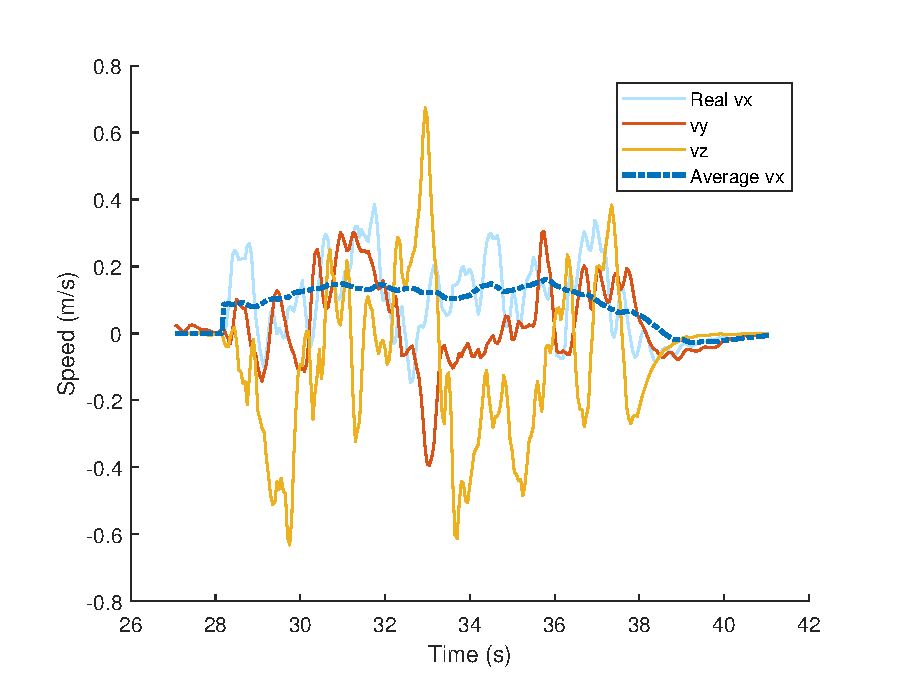
\includegraphics[width=0.9\linewidth]{img/chap5/real_v.eps}
    \caption{The field test results of measurement of velocity at $x$, $y$ and $z$ axis.}
    \label{fig:real_v}
\end{figure}

These results underscore the exceptional transferability and generalization capabilities of the trained controller, highlighting its ability to adapt learned behaviors to real-world settings despite disparities between the simulation and the physical environment. The field tests further emphasize the controller's impressive locomotion performance across various terrains and conditions, providing evidence of its adaptability and robustness in practical scenarios. The outstanding performance observed in the field tests holds significant implications for the power of this methodology enhanced by MBRL. The robot prototype successfully completes the preliminary walking test under real-time execution by utilizing the SAC trained agents.
\chapter{Conclusions}
\label{chap6}
\textit{This chapter summarizes the key findings and contributions of this thesis, providing insights into the achievements and implications of the research conducted. It also outlines the limitations of the study and suggests potential avenues for future research.}

\section{Discussion}
In summary, this research endeavor has sought to unravel the complexities surrounding gait control in soft quadruped robots, with the goal of enhancing understanding and paving the way for more effective control strategies. A systematic exploration of the research questions outlined in this study has yielded valuable insights and findings that contribute significantly to the field of robotics and autonomous locomotion. Additionally, this section will conduct a comprehensive discussion of the research questions outlined in the introduction, with the aim of providing answers and insights based on the research conducted in this study.

\subsection{Answer to Research Questions 1}
The investigation into restricting the state space and designing a surrogate model with high estimation accuracy was instrumental in the pursuit of efficient and accurate simulations and training for soft quadruped robots. This research sought to address this question through two distinct approaches: pattern-defined reinforcement learning and parameterization. These methods provide a solid foundation for efficient and accurate simulations and training, ultimately leading to improved gait control strategies, as shown in Section \ref{Sec:MBRL}. 

The concept of pattern-defined reinforcement learning showed promise as a means to restrict the state space efficiently. By selecting a subset of features based on specific patterns, such as the trot, the study aimed to simplify the state space while retaining essential information. This approach represents a significant step towards efficient simulations and training.

Parameterization introduced a higher-level abstraction into the state-action space by using phases between gait and real motors to parameterize the gaits of quadruped robots. This approach, while complex, holds the potential to simplify the representation of the state space. It has the advantage of capturing critical information about locomotion while streamlining the learning process.

Additionally, it's important to acknowledge the inherent challenges posed by the interconnected nature of the robot's legs. This unique characteristic of soft quadruped robots introduces constraints on the diversity of gaits that can be studied. Unlike robots with independently movable legs, soft quadrupeds exhibit a more synchronized form of locomotion due to their interconnected structure. This limitation restricts the robot's capability to perform certain types of locomotion that may be relevant in real-world scenarios, where adaptability is key.

Given these constraints, our research approach pivoted towards a practical evaluation methodology that prioritized the tangible impact of controllers on the robot's performance in real-world applications. Rather than delving into the intricacies of algorithms in isolation, we directed our focus towards assessing how these controllers influence the robot's stability, walking speed, and cost-of-transport. These metrics serve as practical indicators of a controller's effectiveness in real-world contexts, aligning our research with the practical needs of the field.

This shift in emphasis allowed us to bridge the gap between theoretical developments and real-world deployment, ensuring that our research contributes directly to the enhancement of soft quadruped robots' capabilities in practical scenarios. In essence, our approach recognized the correlation of algorithm design and real-world performance, striving for a holistic understanding of gait control in these unique robotic systems.

\subsection{Answer to Research Questions 2}
Furthermore, the comparative analysis between model-based and model-free reinforcement learning approaches has shed light on the potential of the former in generating superior control agents for soft quadruped robots. The enhancements in stability, walking speed, and cost-of-transport underscore the significance of model-based reinforcement learning as a benchmark in this project. The careful consideration of trade-offs among learning efficiency, simulation accuracy, and long-term planning accuracy has provided essential insights into the quest for optimal gait control policies.

An intriguing fact of our approach resides in the capacity to tailor the controller's behavior to various task objectives through the manipulation of distinct reward functions within the RL framework. By delineating specific reward functions, the RL algorithm learns to optimize the controller for diverse tasks of interest. This adaptability renders the methodology versatile and applicable to a spectrum of scenarios, allowing the robotic system to be endowed with a repertoire of task-specific skills.


\section{Conclusion}
In conclusion, this study embarked on an exploration of enhancing learning efficiency in the context of optimal gait control for soft quadruped robots, with a primary emphasis on addressing the challenges through a MBRL approach. The overall objective was to develop robust gait control policies capable of accommodating the continuous and deformable morphology of the robot while contributing to the advancement of RL control strategies for real-world applications. To substantiate the theoretical framework and proposed methodologies, a series of experimental tests were conducted, ensuring the practical applicability of the research findings. Additionally, a tailored software architecture designed specifically for the soft quadruped robot, SoftQ, was introduced to facilitate the research's objectives.

Nonetheless, it is imperative to acknowledge certain limitations and delimitations that influenced the study's scope. The "sim-to-real gap" constraint underscored the challenges associated with translating simulation results to real-world scenarios, reinforcing the need for a practical evaluation of the proposed gait control strategies. Moreover, the interconnected nature of the robot's legs imposed constraints on the variety of gaits that could be studied, limiting the exploration of certain locomotion strategies relevant to real-world contexts. These limitations necessitated an evaluation focused on the practical impact of controllers on the robot's stability, walking speed, and cost-of-transport, rather than delving into algorithm intricacies.

Delimitations were intentionally set to maintain a concentrated focus on soft quadruped robots, excluding other robotic categories, external environmental factors, hardware design variations, and alternative RL algorithms. This deliberate narrowing of scope aimed to foster an in-depth analysis of the specific challenges related to gait control in the chosen context.

The research methodology encompassed stages of data collection, model-based RL algorithm development, evaluation, analysis, and validation, culminating in the comparison of model-based and model-free RL approaches. Practical validation through physical implementation on SoftQ ensured the relevance of the findings in real-world scenarios. The project also acknowledged ethical and sustainability considerations, emphasizing the responsible use of robotics technology and environmentally-conscious design choices.

In essence, this study contributes to the advancement of soft quadruped robotics by proposing an MBRL approach to gait control, with practical validation underscoring its potential for real-world applications. It is anticipated that the insights gained from this research will pave the way for more efficient and effective RL control strategies, ultimately enhancing the capabilities of soft quadruped robots in various domains, while remaining mindful of ethical and sustainability concerns.

\section{Future Work}
This thesis has explored the context of optimal gait control for soft quadruped robots, uncovering valuable insights and paving the way for further investigations. As with any scientific endeavor, there are promising avenues for future research that can expand upon the knowledge and limitations identified in this study. In this section, the potential directions of future research were outlined for the advancement of soft quadruped robot system.

\subsubsection*{Hardware advancements}
The field of soft robotics is continually evolving, with ongoing developments in soft actuators, materials, and sensors. Future research can explore the integration of state-of-the-art hardware components to enhance the physical capabilities and adaptability of quadruped robots. The continuous evolution of soft robotic materials and actuators presents an opportunity for future research. Investigating the integration of cutting-edge soft robotics hardware, such as novel actuators and sensors\cite{tanShapeEstimation3D2022,tanEdgeEnabledAdaptiveShape2024}, can enhance the physical capabilities and adaptability of quadruped robots, thereby advancing their locomotion control.

\subsubsection*{Multi-terrain adaptation}
Soft quadruped robots should be able to navigate a wide range of terrains, from rugged outdoor environments to indoor spaces. Future research should prioritize the development of control algorithms that enable seamless adaptation to various surfaces. This includes rough, uneven terrains, dynamically changing landscapes, and transitions between different terrain types. Achieving robust multi-terrain adaptation will significantly expand the practical utility of soft quadruped robots across diverse applications.

\subsubsection*{Online learning and adaptation}
The ability of robots to adapt to changing environmental conditions and unforeseen challenges in real-time is crucial. Future research can focus also on developing online learning and adaptation mechanisms that allow soft quadruped robots to continuously update their control policies during operation. This real-time adaptability will be essential for improving performance, responsiveness, and autonomy in dynamic environments.

\subsubsection*{Feedback control to achieve position control}
Incorporating feedback control mechanisms to achieve precise position control is an important area of exploration. Future research can delve into advanced control strategies that enable soft quadruped robots to achieve and maintain specific positions. The significance of this lies in tasks that demand meticulous positioning, such as precise robotic manipulation, obstacle avoidance, and navigating through confined spaces. By developing control techniques that seamlessly incorporate precise position control into the skill set of soft quadruped robots, we can open up new possibilities for their application in a wider array of scenarios.

\subsubsection*{Robustness and fault tolerance}
Ensuring the robustness and fault tolerance of soft quadruped robots is critical for real-world applications. Future research can investigate robust control strategies capable of withstanding disturbances, uncertainties, and unexpected environmental changes. Additionally, the development of fault-tolerant control mechanisms will be essential for handling hardware failures or damage, ensuring the reliability and safety of these robots in challenging scenarios.

\subsection{Sustainability and Ethical Considerations}
In a world increasingly concerned with environmental impact, the notion of environmental sustainability is more relevant than ever. In the context of this thesis, significant consideration was given to the COT metric as a guiding factor in the design of the controller. Emphasis was placed on the role of energy efficiency in the performance of soft quadruped robots, with the objective of creating controllers that enhance the robot's endurance while minimizing its environmental impact.

The choice of materials and manufacturing techniques applied in this research proved to be highly advantageous in achieving these goals. The utilization of compliant and soft materials was aligned with the inherent characteristics of quadruped locomotion and contributed to improved energy efficiency. These materials facilitated better energy absorption and recovery during the robot's gait, leading to reduced energy losses and enhanced overall efficiency.

Furthermore, the incorporation of advanced 3D printing methods enabled the creation of intricate and customized components for the soft quadruped robot. This level of manufacturing precision not only minimized material wastage but also bolstered structural integrity, further supporting the overarching objectives of sustainability and energy efficiency. These considerations are not mere addenda but foundational principles that should guide every stage of robotic development.

Crucially, regulatory frameworks serve as the scaffolding upon which sustainability and ethics are built. Collaborative efforts among governments, industry bodies, and researchers are essential to craft standards and guidelines that embody these principles. Such frameworks are not restrictive but liberating, providing a clear roadmap for the responsible development and deployment of soft quadruped robots.

As soft quadruped robots become integrated into society, ethical considerations, including privacy, safety, and their impact on employment, require careful examination. Future research should also delve into these ethical dimensions to ensure the responsible deployment of these robots.

\subsection{Final Words}
In these final words, it is crucial to acknowledge the collaborative efforts of researchers, engineers and innovators who continue to push the boundaries of robotics. The journey to master gait control in soft quadruped robots is ongoing, with numerous challenges and opportunities awaiting exploration.

In the grand scheme of scientific exploration, this research represents a small but significant stride toward unlocking the full potential of soft quadruped robots. It is our hope that the knowledge gained here will inspire further research and innovation, ultimately leading to the realization of highly capable and versatile soft quadruped robots that can navigate the complexities of our ever-changing world.

In closing, this thesis marks not an end, but rather a new beginning in the journey to harness the untapped potential of soft quadruped robots. May our collective efforts continue to drive progress, pushing the boundaries of what these remarkable machines can achieve.








% \include{content}
%TC:ignore 
\newpage
% \addcontentsline{toc}{chapter}{References}
% \pagestyle{empty}
\setstretch{1}
% \fontsize{5}{0}
\footerfont
\printbibliography[heading=bibintoc]

\newpage
\appendix
\newpage

\etocdepthtag.toc{mtappendix}
\etocsettagdepth{mtchapter}{none}
\etocsettagdepth{mtappendix}{subsection}
\etoctocstyle{1}{Appendix - Contents}
\tableofcontents
\pagestyle{plain}
\newpage
\pagenumbering{arabic}

\chapter{First Appendix}
This is only slightly related to the rest of the report

\begin{figure}[ht]
    \centering
    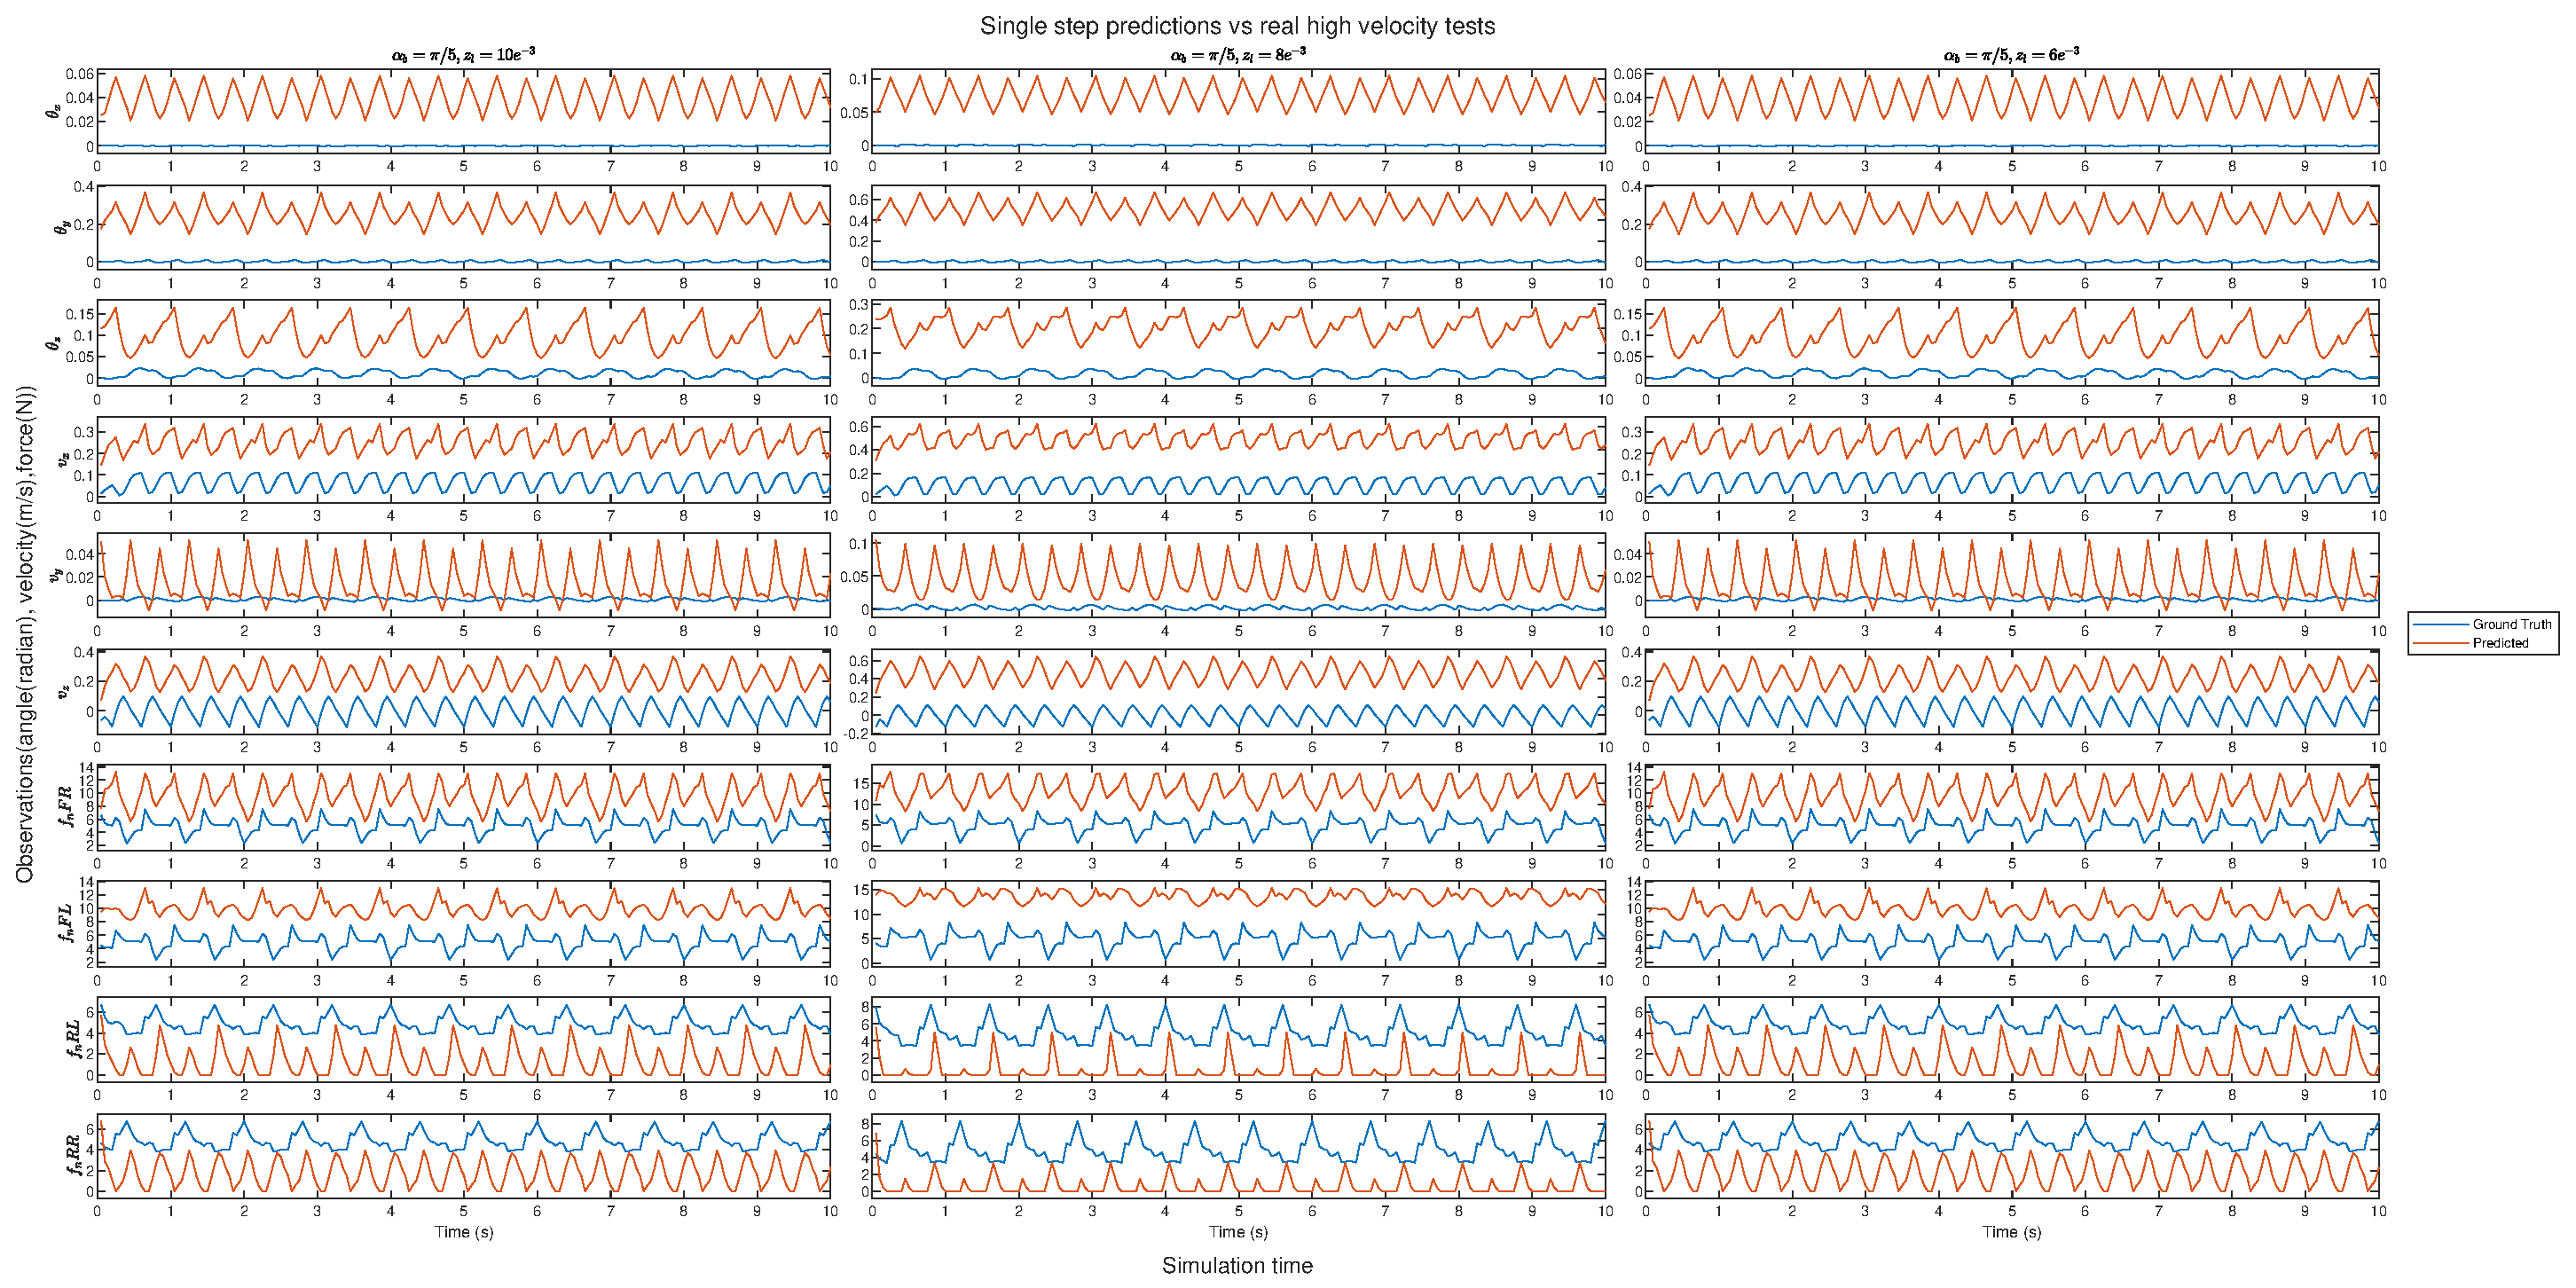
\includegraphics[width=\linewidth]{img/AppA/rq1_pi51_1.eps}
    \caption{Schematic illustration of hypothetical \ac{CPG} structure for mammalian movement control, reproduced from Li et al.\cite{liHumanoidsLearningWalk2013}}
\end{figure}


\chapter{Second Appendix}
this is the information


\newpage
% This is the last page of the document
\thispagestyle{empty}
\AddToShipoutPictureBG*{%]
    \AtPageLowerLeft{%
        \includegraphics[width=1.0\paperwidth]{setup/img/kth-footer.png}
    }%
}

\PlaceText{140mm}{272mm}{\color{white}\fontsize{10}{0} TRITA – ITM-EX 2023:XXX }


\PlaceText{20mm}{282mm}{\color{white}\fontsize{12}{0}\sffamily \href{www.kth.se}{www.kth.se}}

%TC:endignore 
\end{document}
